\documentclass[11pt,a4paper]{article}

\usepackage[utf8x]{inputenc}   % omogoča uporabo slovenskih črk kodiranih v formatu UTF-8
\usepackage[slovene]{babel}    % naloži, med drugim, slovenske delilne vzorce
\usepackage{url}
\usepackage{graphicx}

\usepackage{hyperref}

\title{Asistent Slivko \\
\large Seminarska naloga za Informacijske sisteme}
\author{
Jernej Habjan, 63150106  \\
Matic Vrtačnik, 63150317 \\
\ \\
Fakulteta za računalništvo in informatiko Univerze v Ljubljani
\date{\today}         
}


\begin{document}
\maketitle



\section{Spletna aplikacija}

Spletna aplikacija je dosegljiva na naslednjem spletnem naslovu: 
\href{http://asistentslivko.azurewebsites.net/}{Spletna aplikacija Asistent Slivko}.
Aplikacija nam z Google Maps ponuja prikaz leta iz enega kraja v drug, pri katerem lahko ta let tudi naročimo preko forme, ki uporabi storitev, da v podatkovno bazo vpiše nov let.
Za prijavo uporabljava Google Login, kjer se Googlov id vpiše v bazo na Azure in tega uporabjava za pridobivanje in pisanje podatkov.
Prav tako ima vsak uporabnik določene pravice (uporabnik, admin), kjer lahko admin na glavni strani izbira uporabnika, od kogar hoče pregledati vsa naročila.
Uporabnik si lahko spremeni prikazno ime (Update)

Posamezno svoje (vsi) ali tuje (admin) preteklo naročilo lahko tudi podrobno pregleda tako, da na glavni strani izbere let, odpre se mu pa nova stran, kjer vidi vse podatke o samem letu, prav tako pa vidi potnike, ki so v tem naročilu nastopali.

Prav tako lahko prejšna naročila izbrišemo (Delete).

Nov let pa ustvarimo tako, da izpolnimo vse podatke na strani Planiranja in potrdimo naročilo leta. Tu nam izpiše končno ceno, prav tako pa lahko vnesemo alternativno plačilno sredstvo - kartica.

\section{Storitve}
Aplikacija ima 3 storitve:
\begin{itemize}
	\item Google Login~\cite{signIn} - S katerim se lahko prijavimo v aplikacijo z Googlovim računom.
	\item Google Autocomplete\cite{autocomplete} - Polje ki se samo izpolnjuje, ko pišemo vanj kraje. Ista funkcionalnost kot vnosno polje na Google Maps.
	\item REST storitev za upravljanje podatkovne baze na Microsoft Azure.
\end{itemize}
Storitve REST so razdeljene na 2 skupini - Podatki oseb in podatki o naročilu.

\subsection{Podatki oseb}

	\begin{itemize}
		\item Tu lahko vrnemo podatke o uporabniku, če podamo googleID
		\item Dodajanje novega uporabnika
		\item Izbris uporabnika
		\item Posodobitev uporabnika
		\item Vrnitev vseh potnikov v določenem letu
		\item Vloga uporabnika (user, admin)
	\end{itemize}
\subsection{Podatki o naročilu}

	\begin{itemize}
		\item Vračanje vseh naročil uporabnika
		\item Vračanje točno določenega naročila
		\item Dodajanje naročila
		\item Brisanje leta
	\end{itemize}

\section{Podatkovna baza}
S podatkovno bazo, ki je dostopna na portalu Microsoft Azure, upravljamo preko REST storitev.
Storitve kličemo z odjemalca android z uporabo knjižnice Volley (Pokrite vse CRUD zahteve)

\begin{figure}[htb]
	\centerline{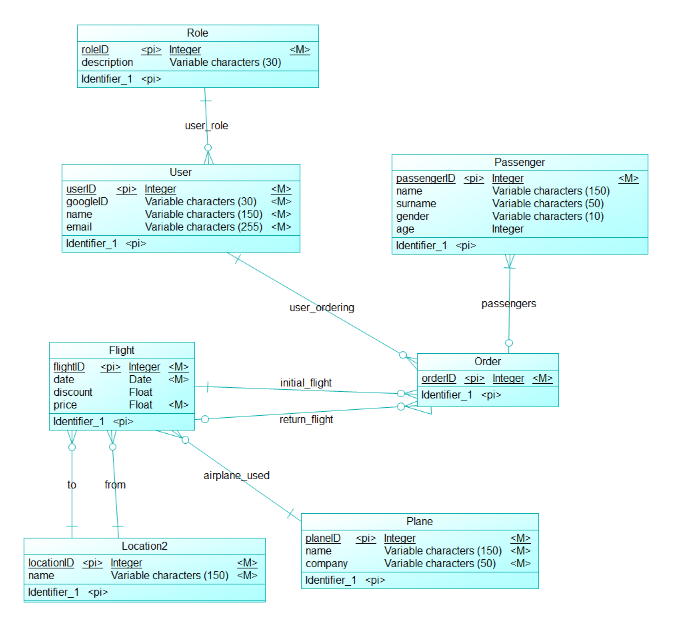
\includegraphics[width=1.0\textwidth]{bazaVAzure.png}}
	\caption{Konceptualni model podatkovne baze v Microsoft Azure}
	\label{sl:koncept}
\end{figure}
\begin{itemize}
	\item Za registracijo uporabnika z Googlovim ID v lastno podatkovno bazo,
	\item Pridobitev informacij o uporabniku iz baze,
	\item Vnos in pridobitev informacij o naročilu, letu, letalu in potnikih v in iz baze,
	\item Preimenovanje uporabniškega imena,
	\item Izbris prejšnih potovanj

\end{itemize}


\section{Odjemalec android}

Okna pri aplikaciji so fragmenti, ki so povezani preko glavne aktivnosti, skozi katero si izmenjujejo podatke.
Aplikacija ima poleg pomikanja skozi okna z gumbi tudi navigacijsko okno, s katerim se lahko vrnemo na različne zaslone, pri vnašanju potnikov in informacij o letu nas pa aplikacija sama vodi skoz njih.
Komunikacija med fragmenti poteka z Bundle preko Vmesnikov, ki jih implementira glavna aktivnost.


Aplikacija je bila že delno izgrajena za predmet Uporabniški vmesniki, kjer so bili ustvarjeni osnovni fragmenti in njihova komunikacija.
Za implementacijo Google Sign-In sva si pomagala z s predlogo, objavljeno na Google GitHub repozitoriju, ki vsebuje primer fragmenta z implementirano prijavo~\cite{loginSample}.
Prav tako sva si veliko pomagala s stranjo Stack Oveflow za razreševanje problemov~\cite{stack}.
Aplikacija je izdelana v programskem jeziku Kotlin.

\section{Opis oken}
\subsection{Uporabnik}
Okno uporabnik se pojavi, ko v aplikacijo nismo prijavljeni z Googlovim računom.
Tu se prijavimo z Google sign-in. Prav tako lahko tu spremenimo svoje prikazno ime, ki posodobi zapis v bazi.

\subsection{Potovanja}
V oknu se nam prikažejo vsa naša prejšna potovanja, ki jih lahko z gumbom odpri pregledamo, prav tako pa jih lahko zbrišemo.
Na temu oknu lahko tudi pritisnemo gumb za dodajanje novega naročila.

\subsection{Nakup}
Ob pritisku gumba za dodajanje novega naročila nas aplikacija privede na okno nakup, kjer imamo za vnos odhoda in prihoda dva Google Autocomplete fragmenta, v katera vnesemo kraj.
Vnesemo še ostale podatke in nadaljujemo na določanje potnikov.

\subsection{Potniki}
Tu se nam izpišejo vsi potniki, ki spadajo k temu letu. Če smo si ogledali že opravljen let, bomo tu videli potnike, če pa ustvarjamo nov let, moramo pa dodati nove potnike skozi novo okno vnos potnika

\subsection{Vnos potnika}
Tu vnesemo osnovne lastnosti potnika kot ime, priimek, spol in leto rojstva.
Ob zaključku se ta potnik vnese v tabelo na oknu Potniki.

Ko imamo vnešenega vsaj enega potnika, lahko nadaljujemo na zaključek plačila.

\subsection{Plačilo}
Tu nam izpiše število potnikov in lahko izberemo kot plačilo kreditno kartico, za katero moramo podatke tudi vnesti.
Ob zaključku plačila, se naredi vnos v podatkovno bazo za celoten let.


\section{Slike}

\begin{figure}[htb]
\centerline{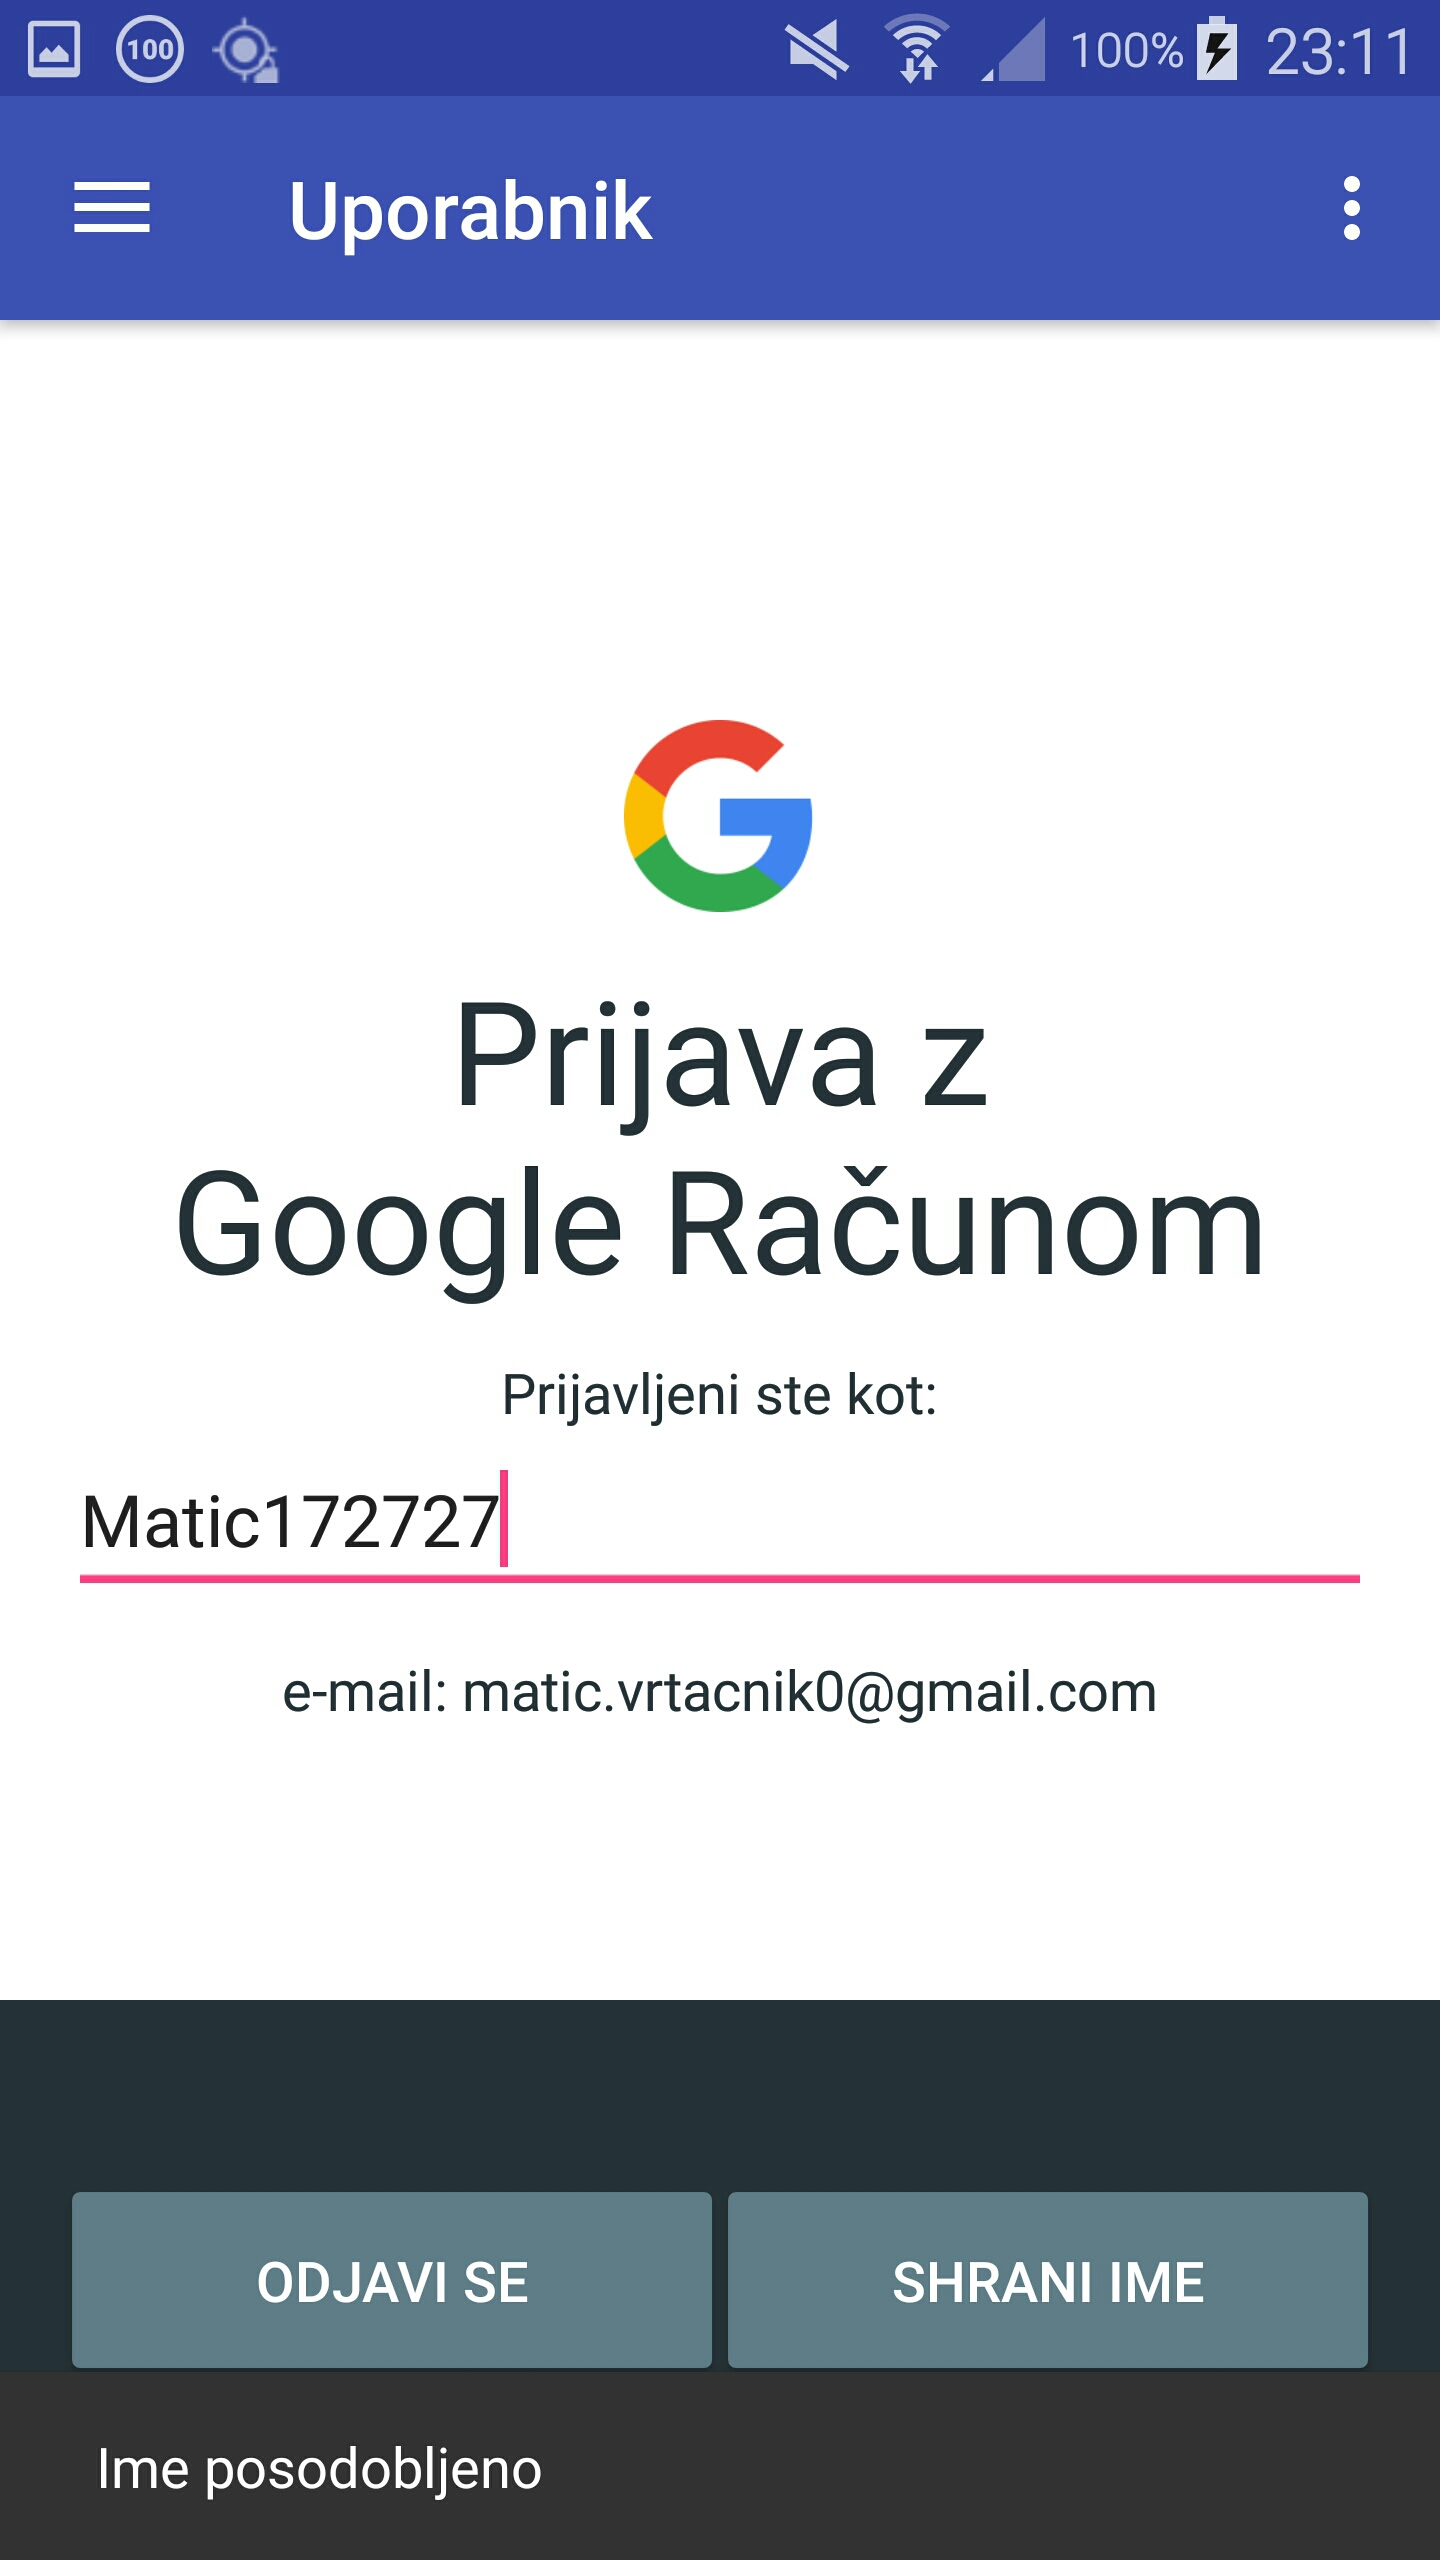
\includegraphics[width=1.0\textwidth]{GUI/login.jpg}}
\caption{Okno za prijavo uporabnika in spreminjanje imena}
\label{sl:koncept}
\end{figure}

\begin{figure}[htb]
	\centerline{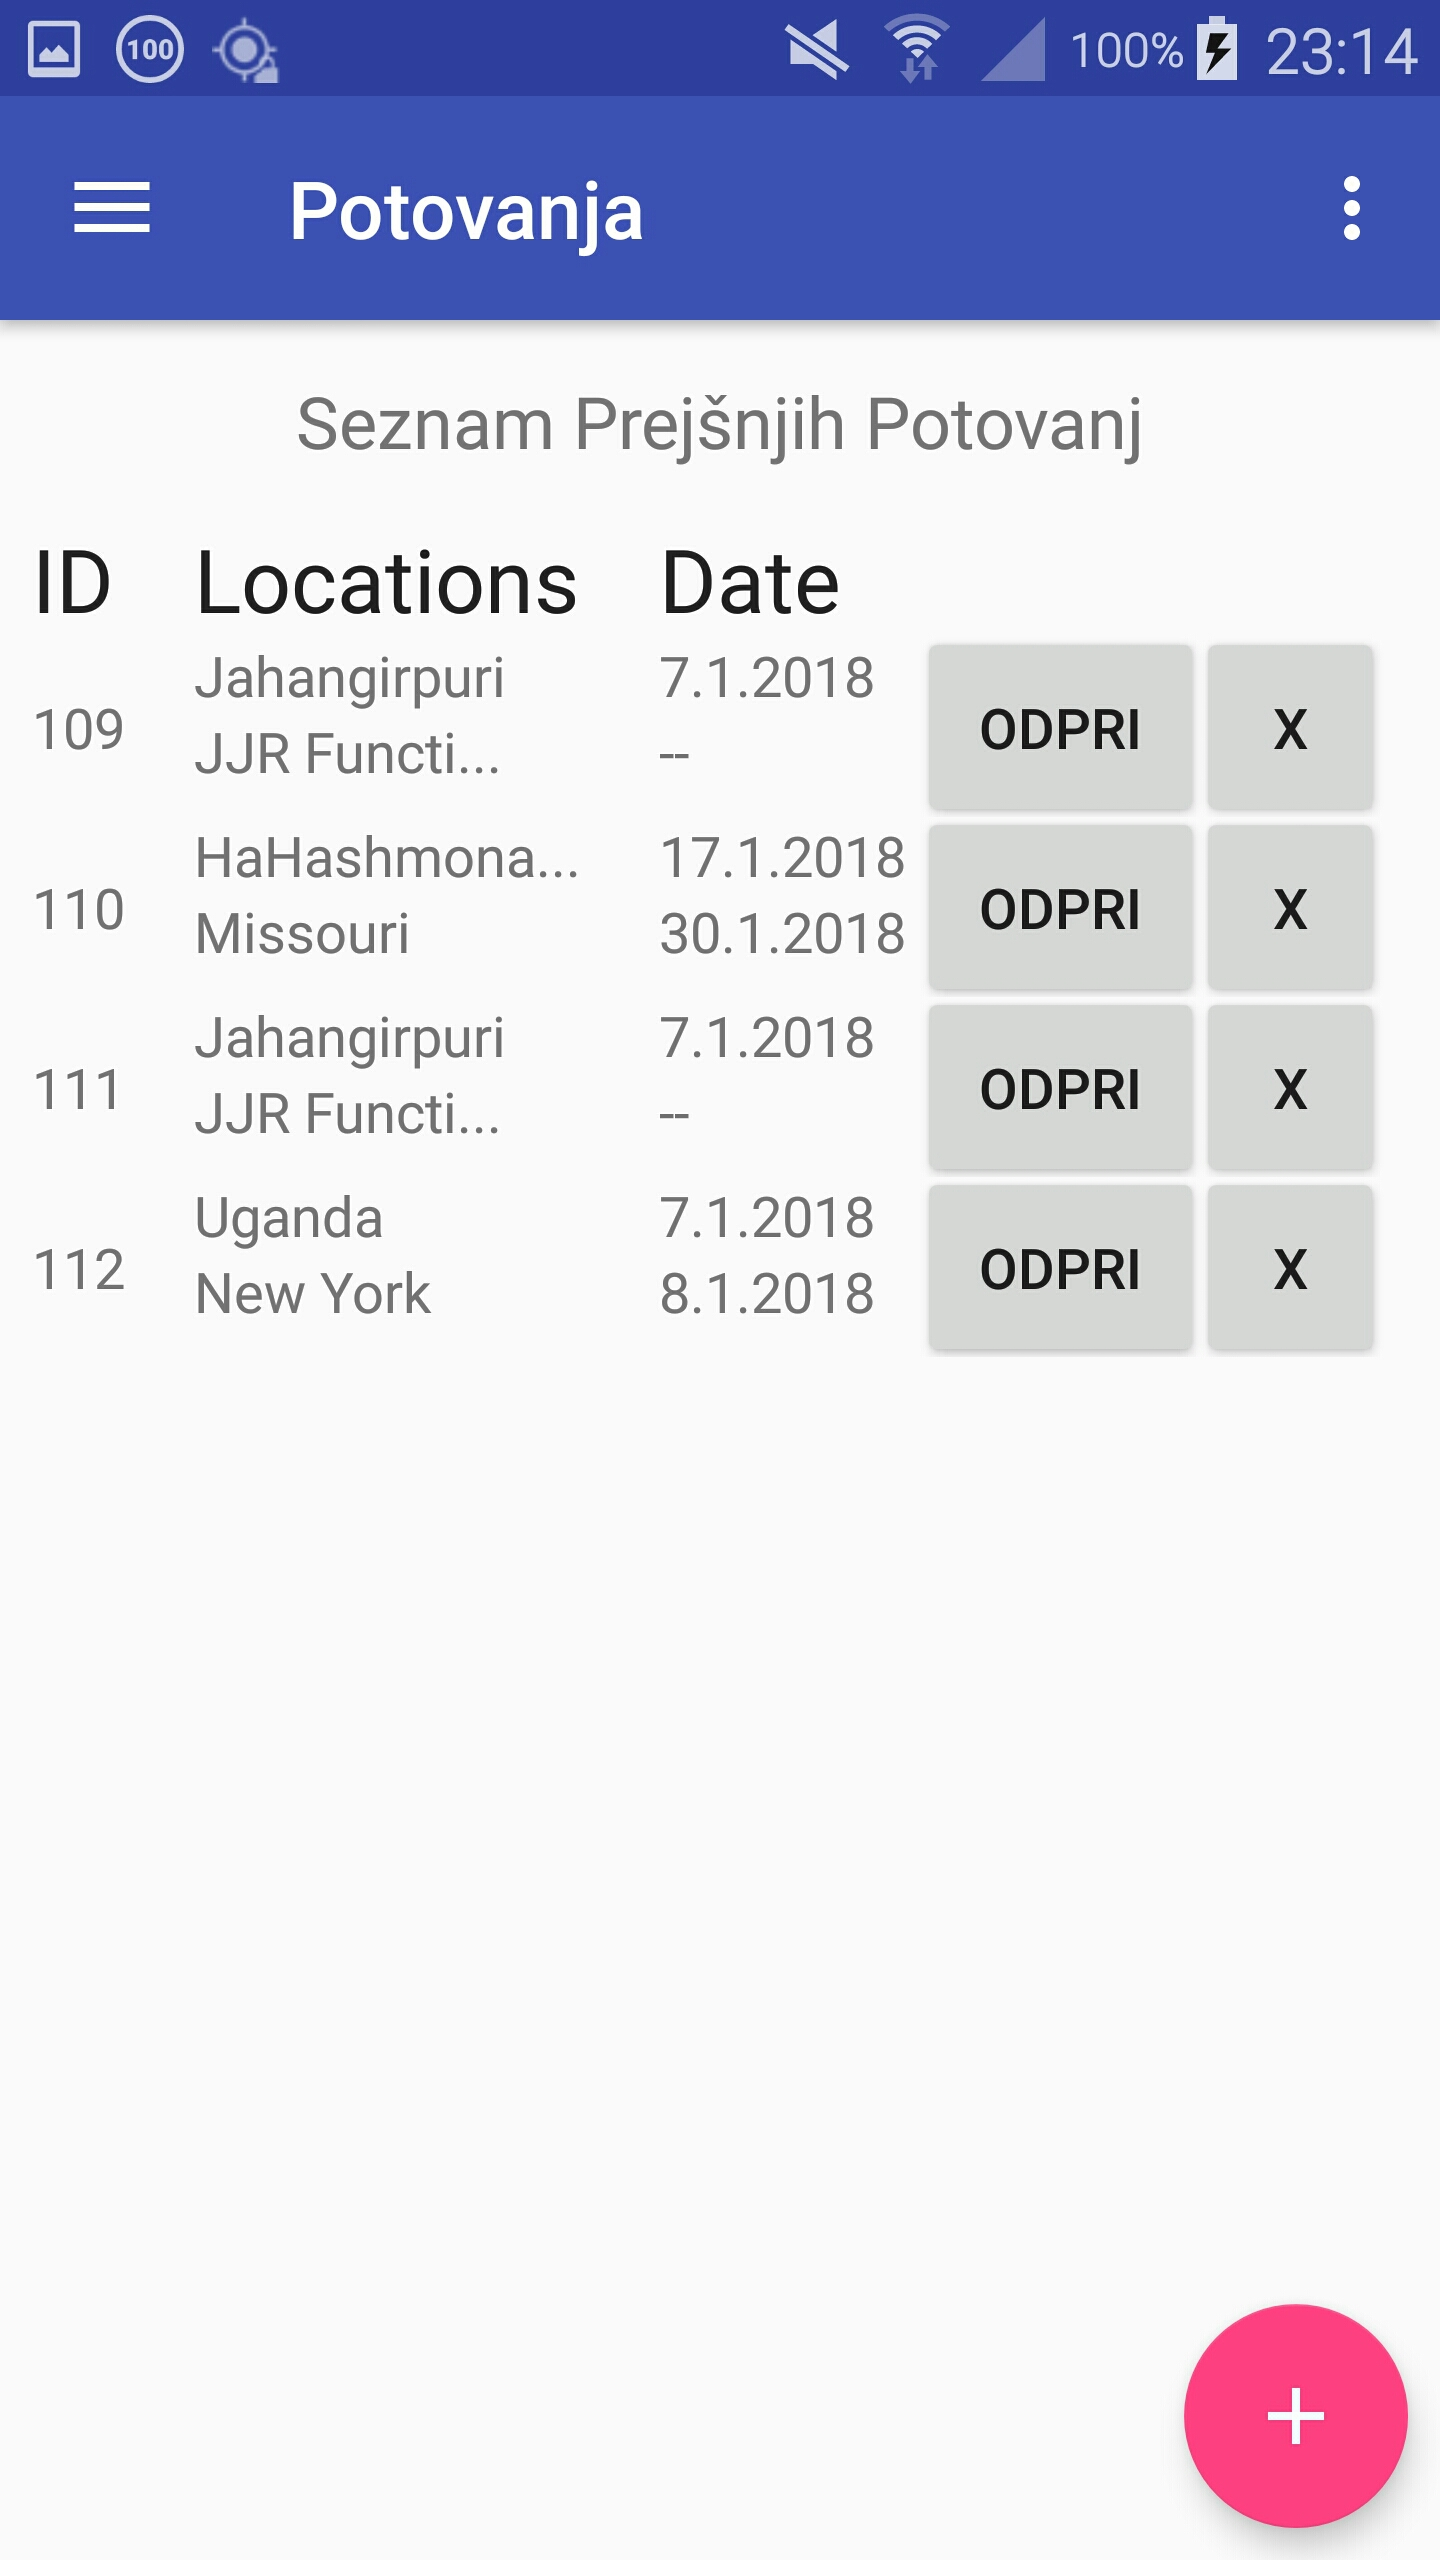
\includegraphics[width=1.0\textwidth]{GUI/potovanja.jpg}}
	\caption{Prikaz prejšnih letov}
	\label{sl:koncept}
\end{figure}

\begin{figure}[htb]
	\centerline{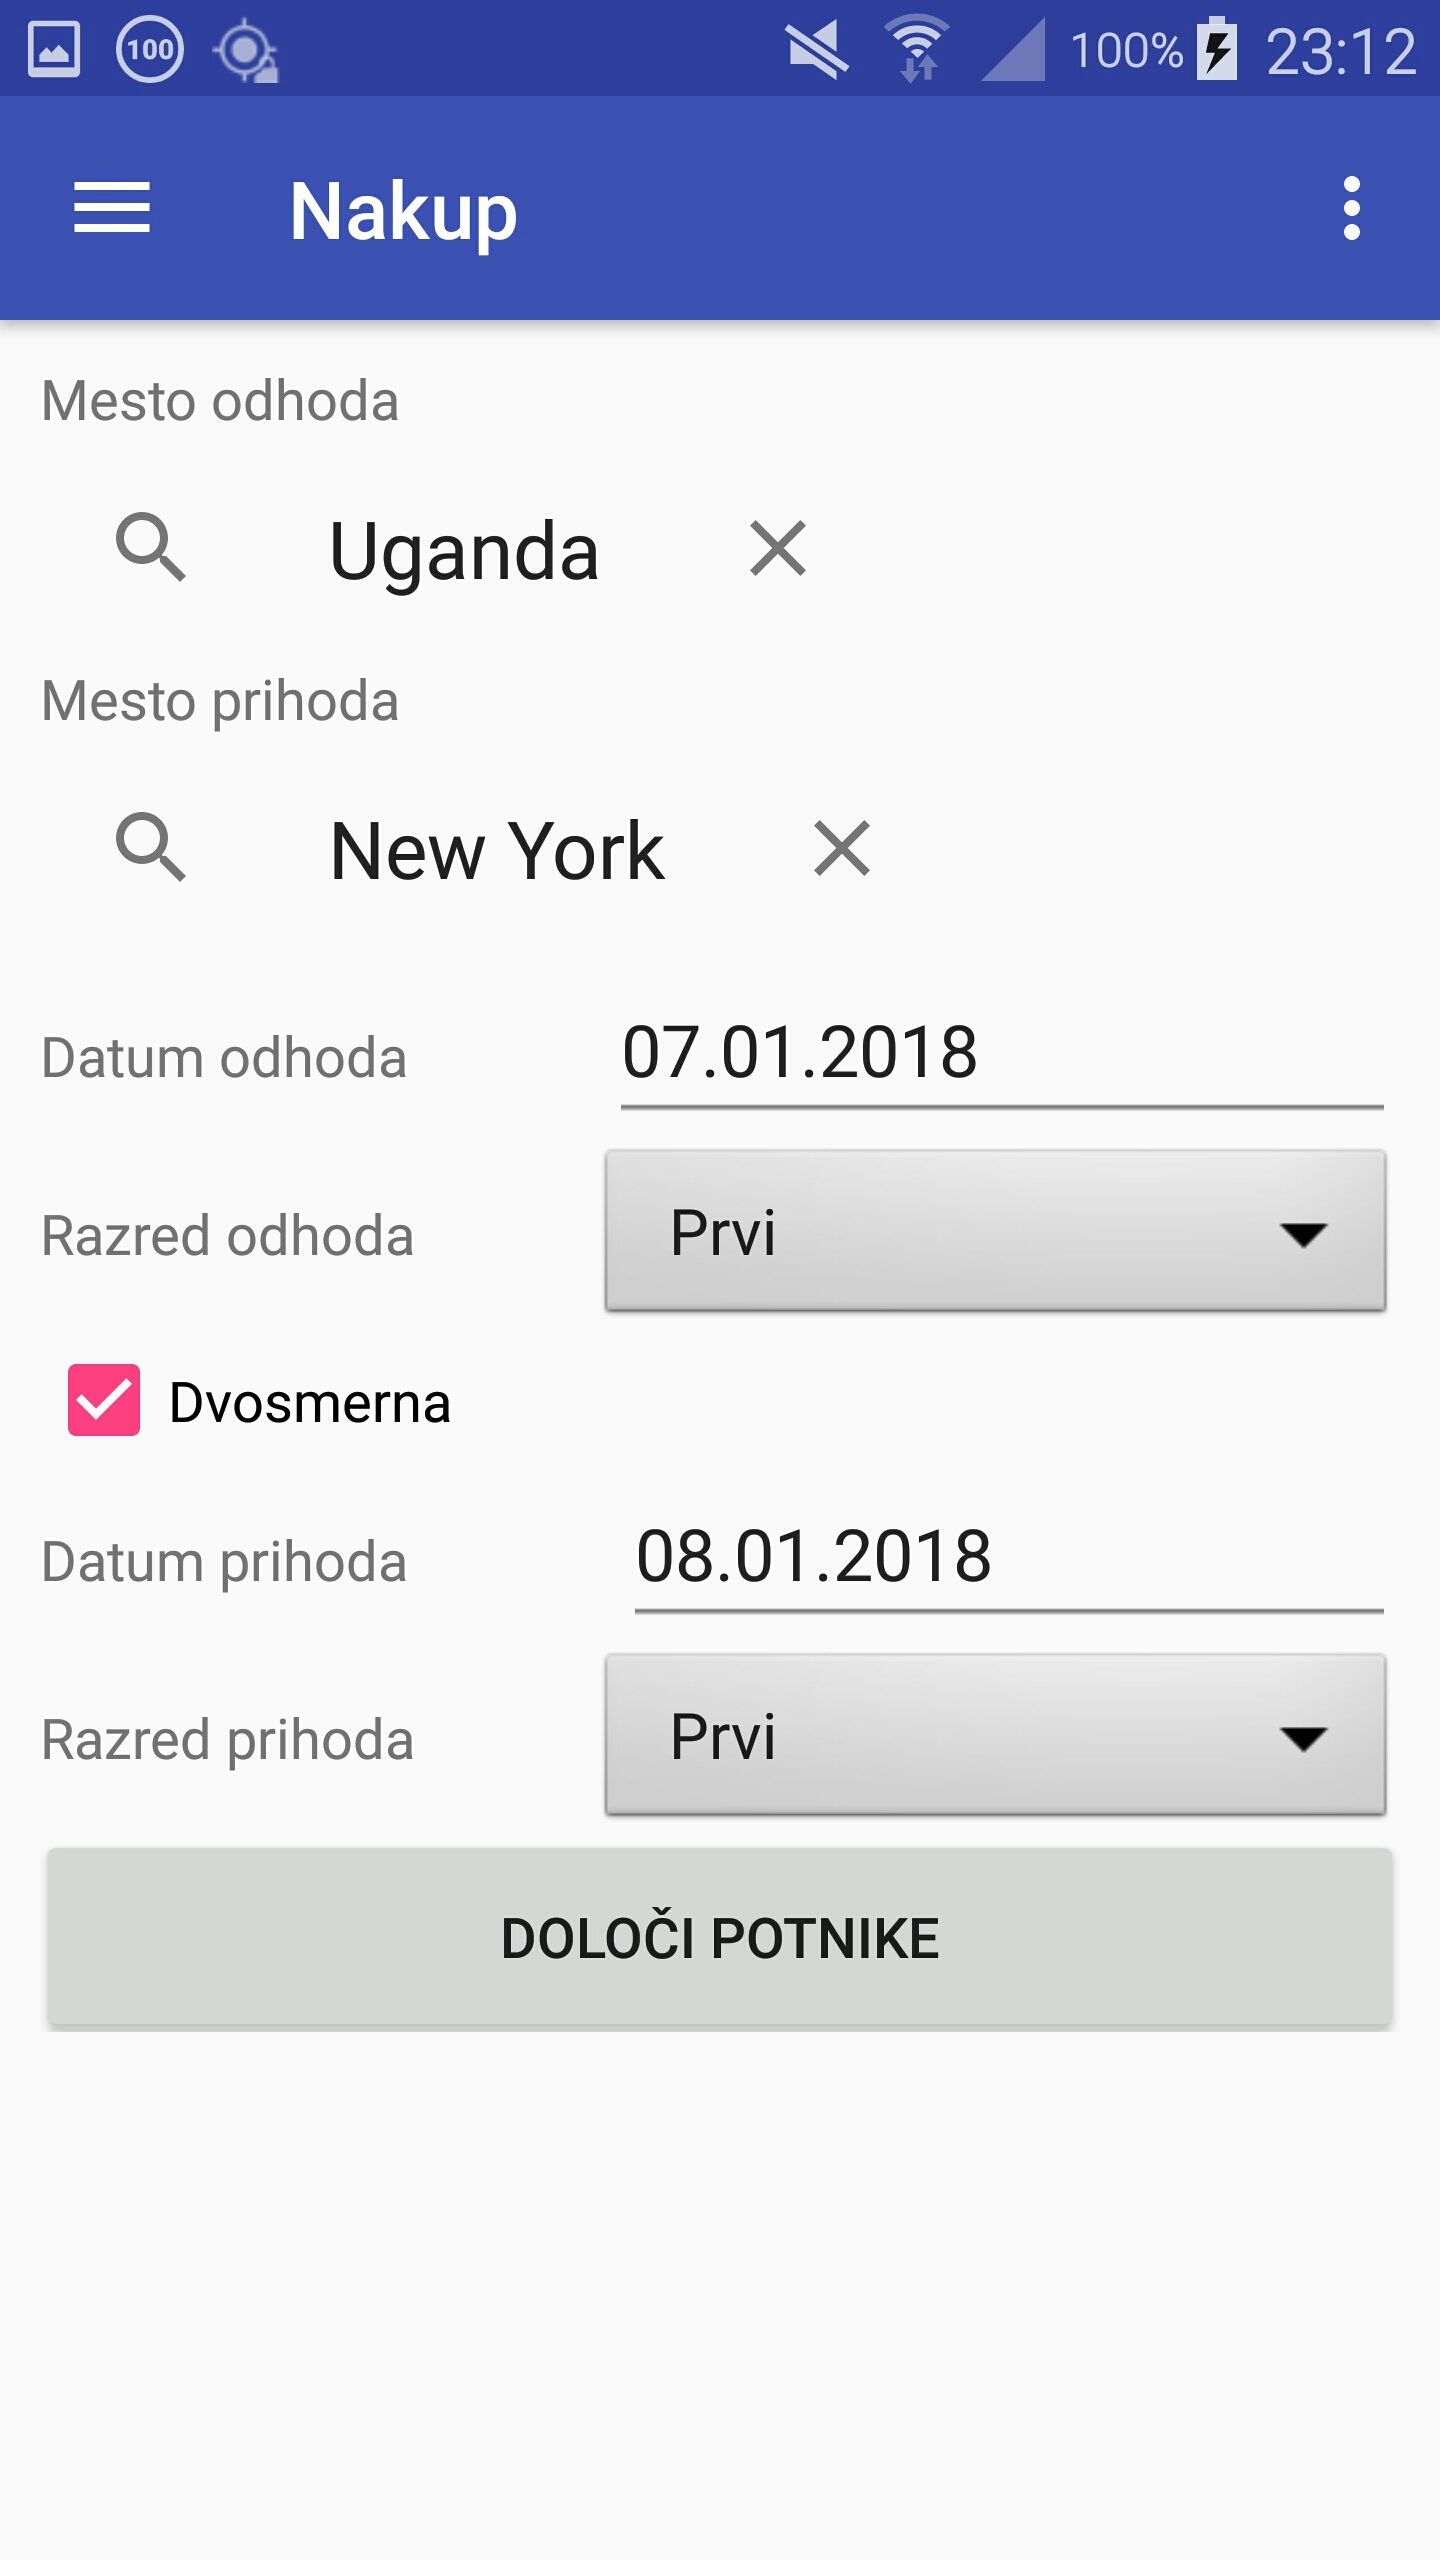
\includegraphics[width=1.0\textwidth]{GUI/nakup.jpg}}
	\caption{Okno za določitev leta - vsebuje Google Autocomplete}
	\label{sl:koncept}
\end{figure}



\begin{figure}[htb]
	\centerline{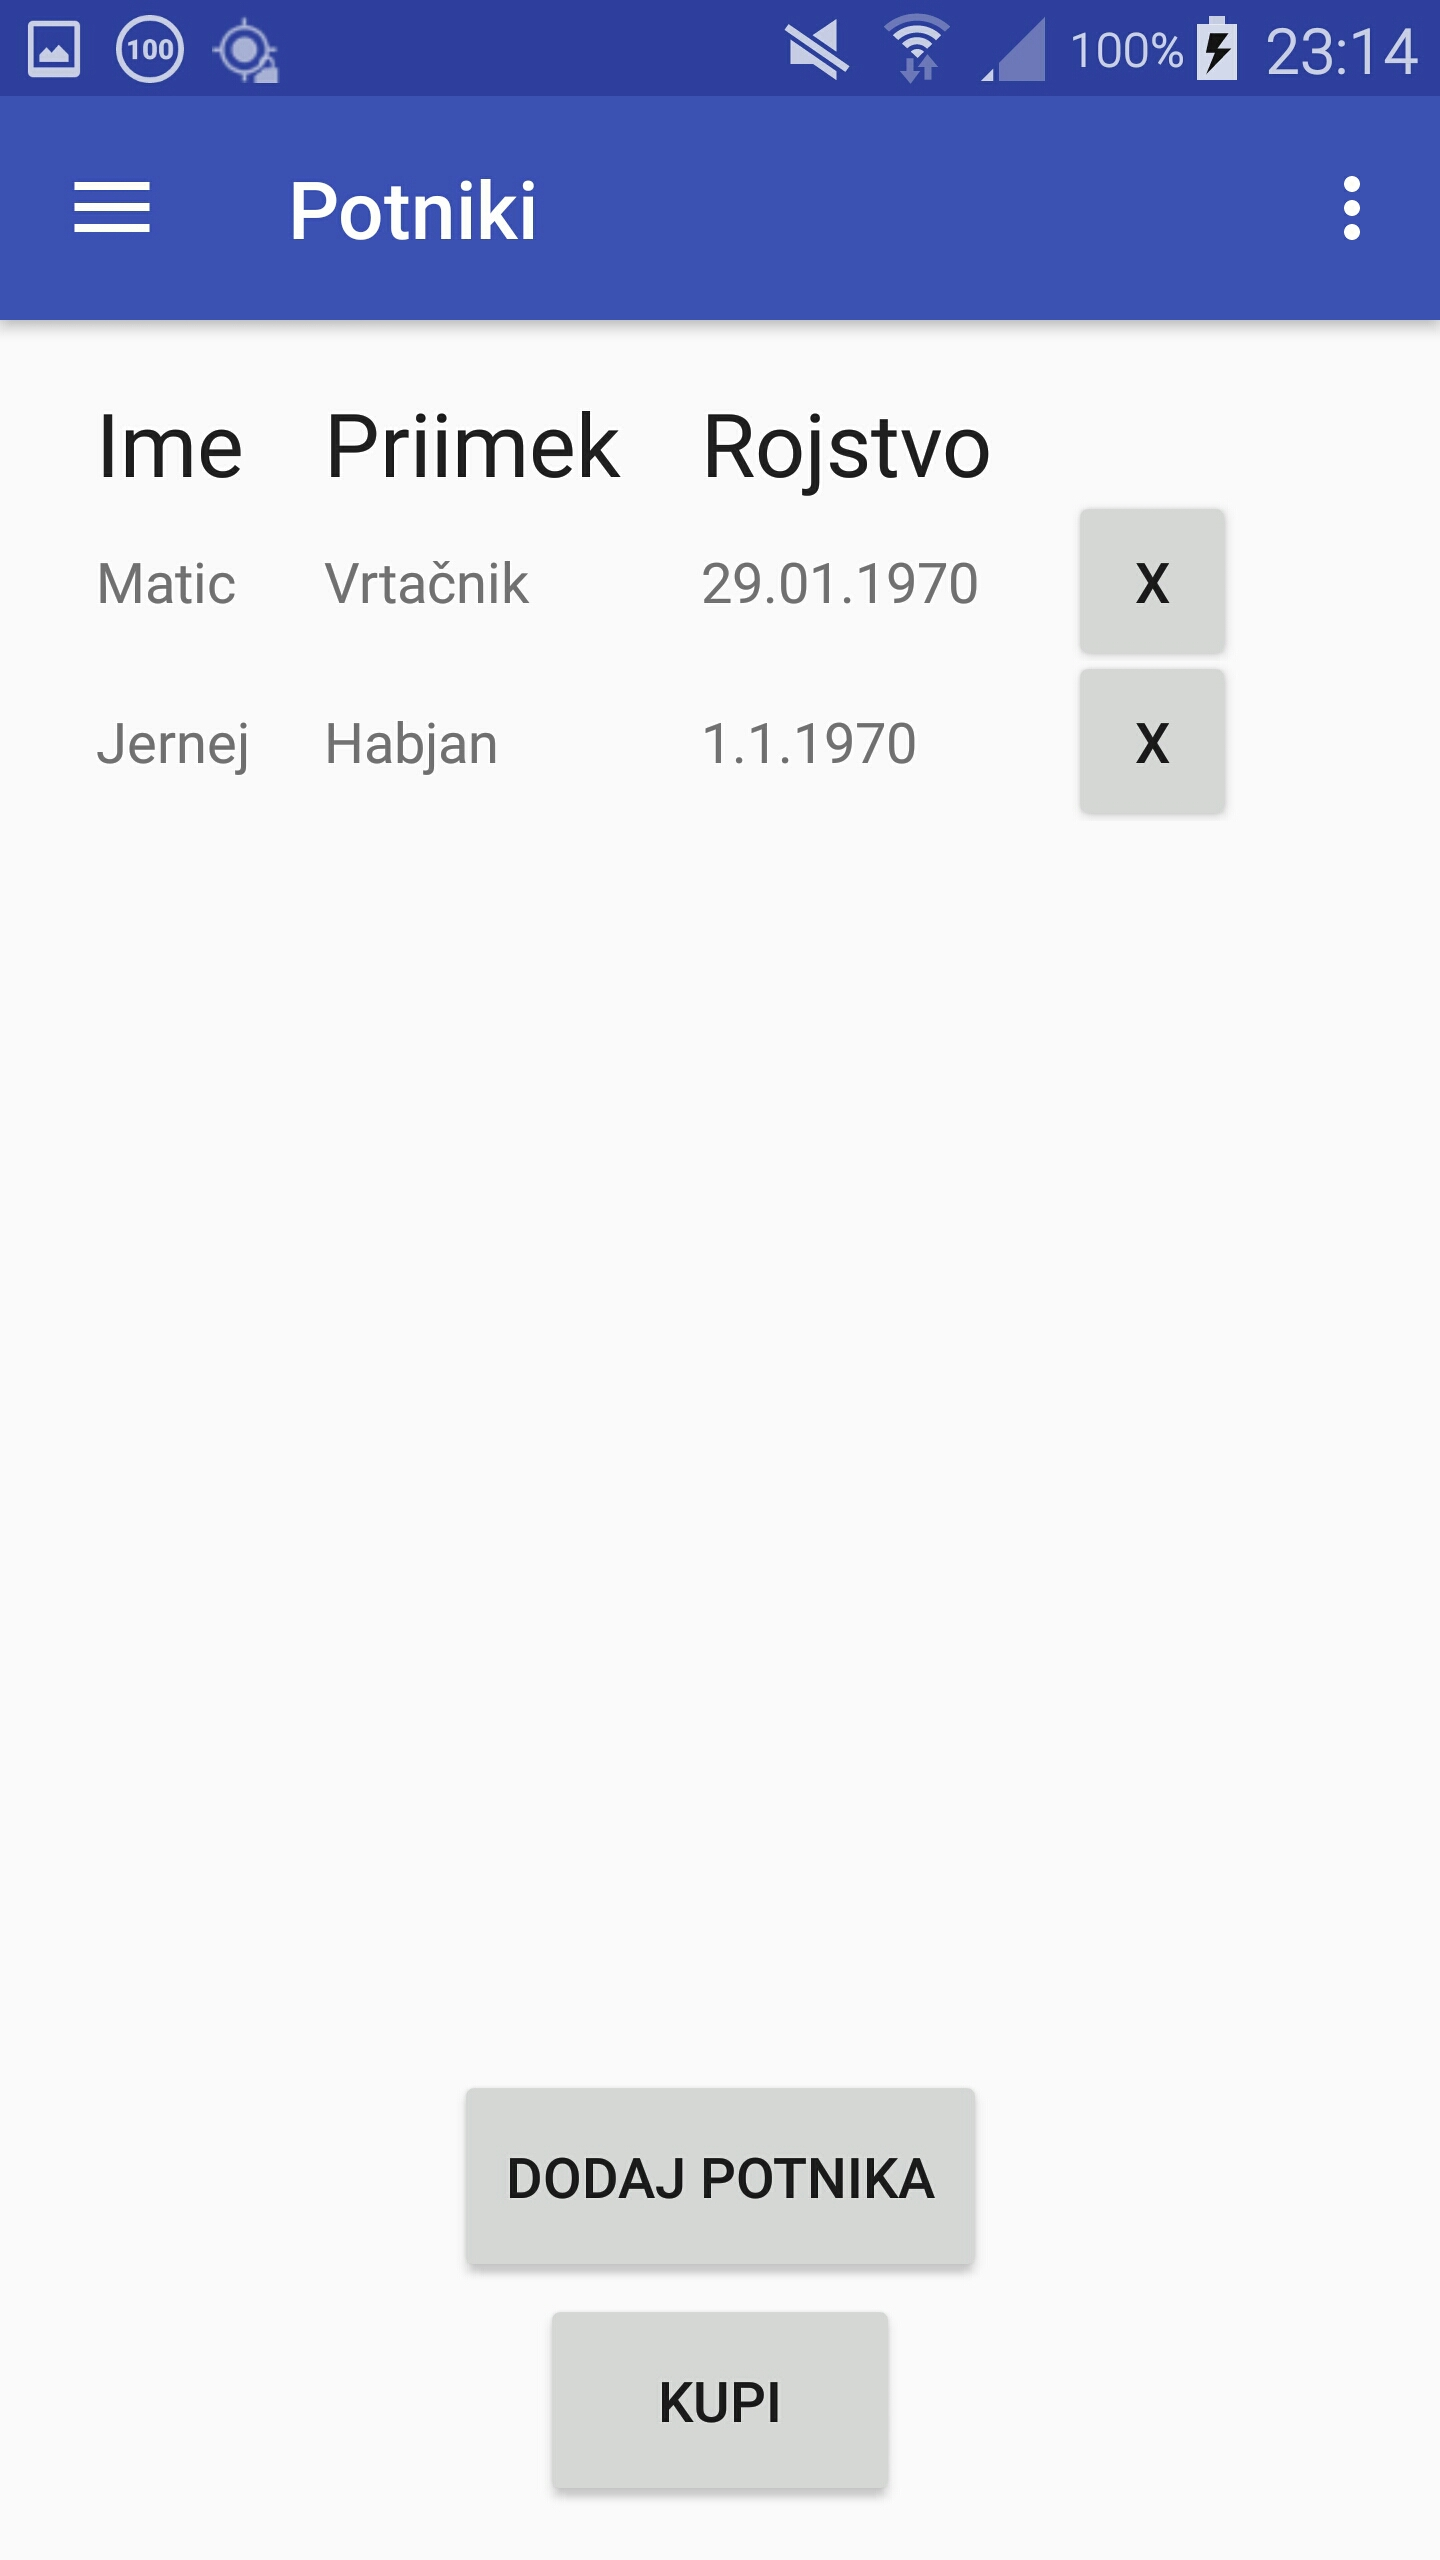
\includegraphics[width=1.0\textwidth]{GUI/Potniki.jpg}}
	\caption{Prikaz vnešenih potnikov}
	\label{sl:koncept}
\end{figure}


\begin{figure}[htb]
	\centerline{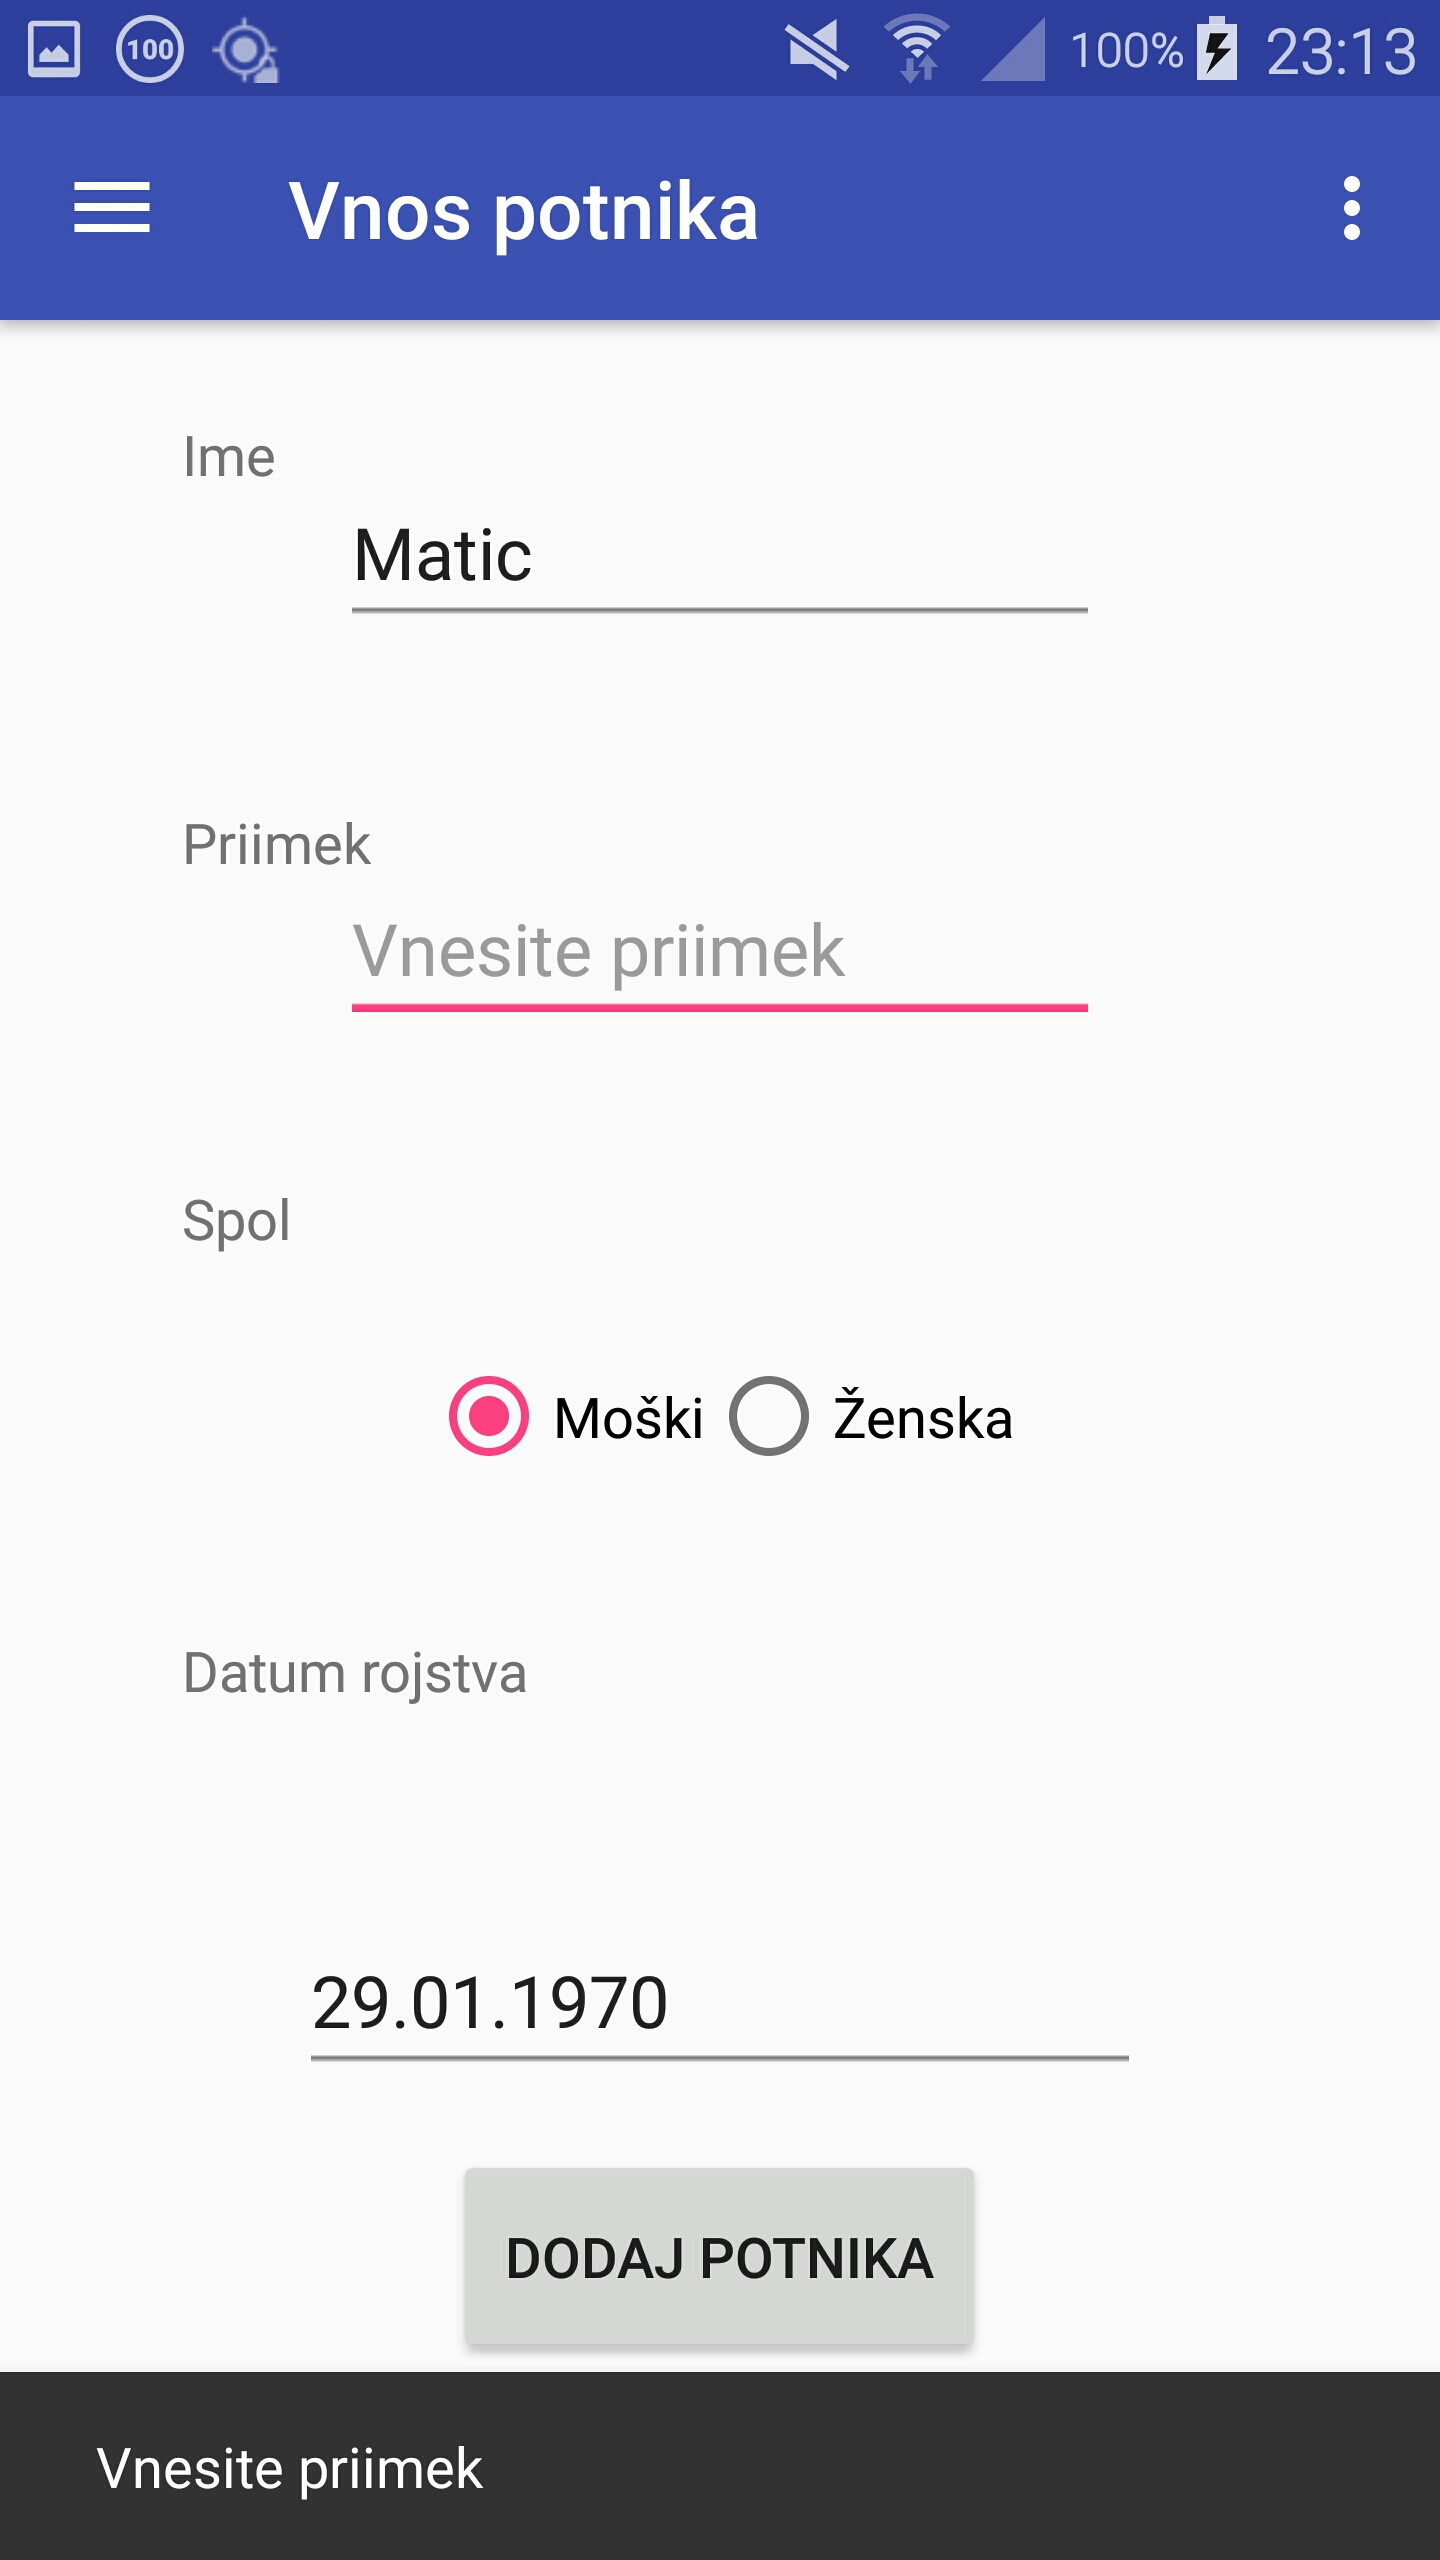
\includegraphics[width=1.0\textwidth]{GUI/vnosPotnika.jpg}}
	\caption{Vnos potnika}
	\label{sl:koncept}
\end{figure}


\begin{figure}[htb]
	\centerline{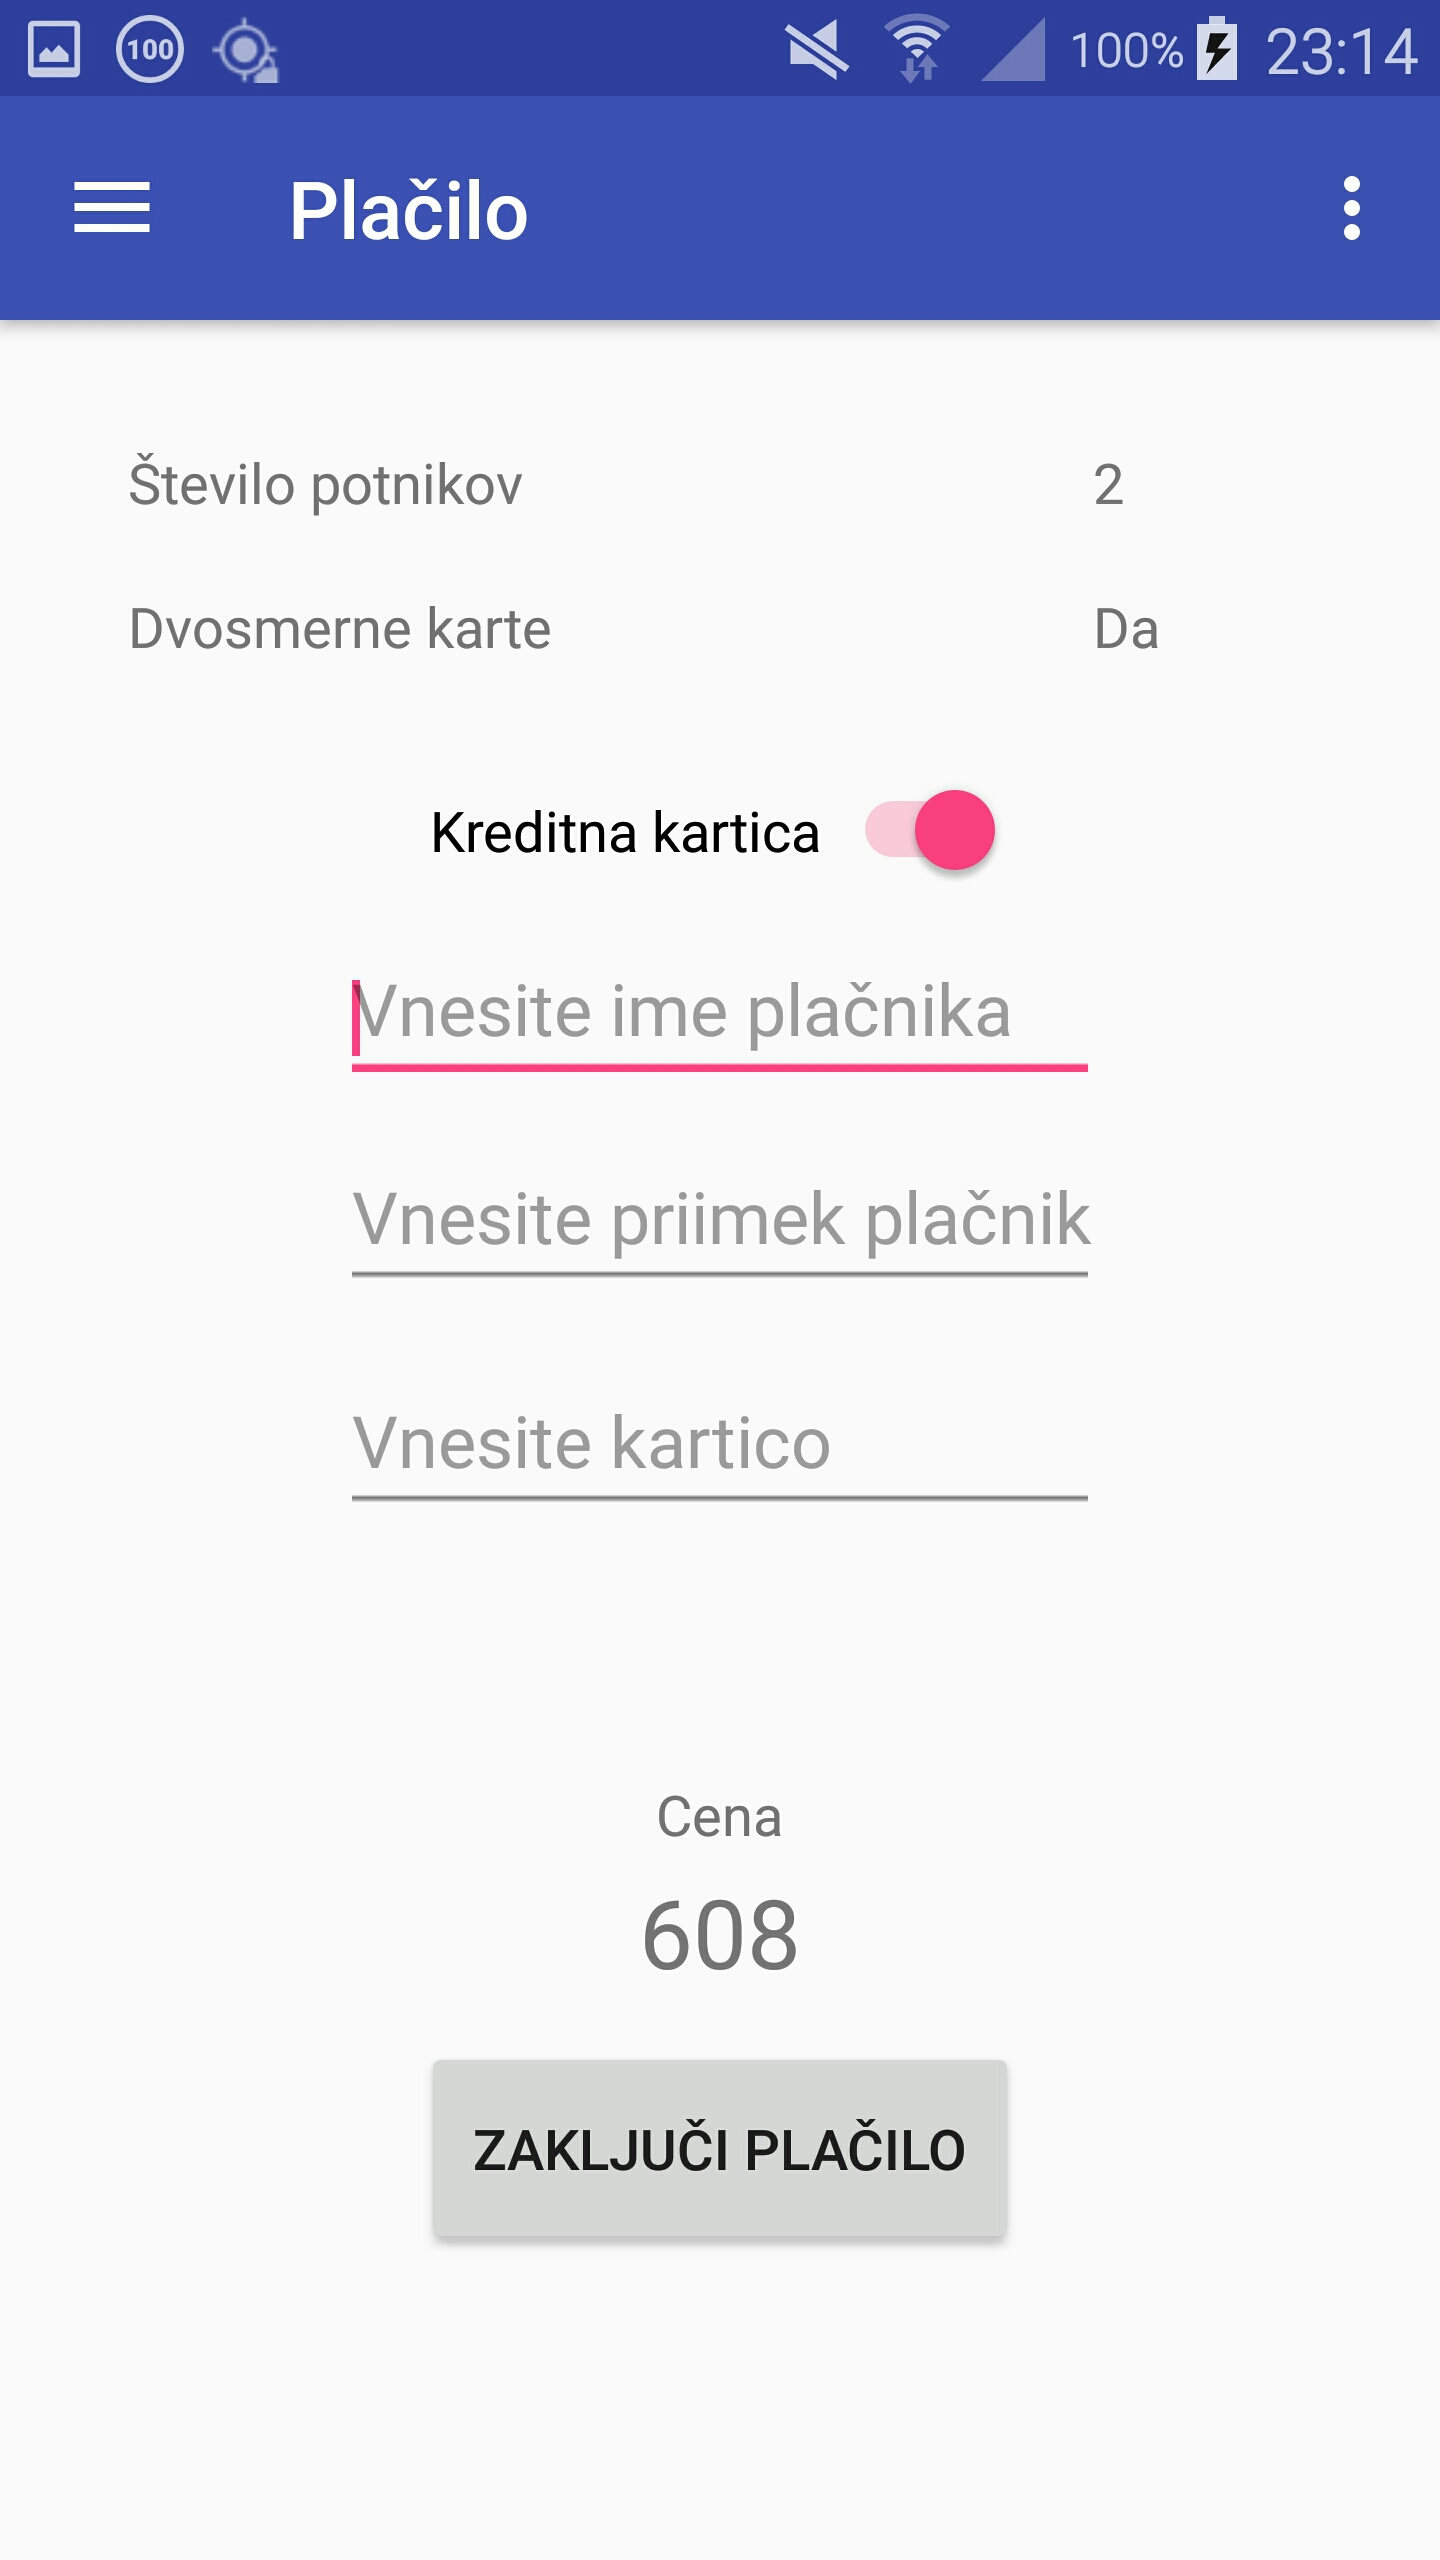
\includegraphics[width=1.0\textwidth]{GUI/placilo.jpg}}
	\caption{Plačilo}
	\label{sl:koncept}
\end{figure}

\begin{figure}[htb]
	\centerline{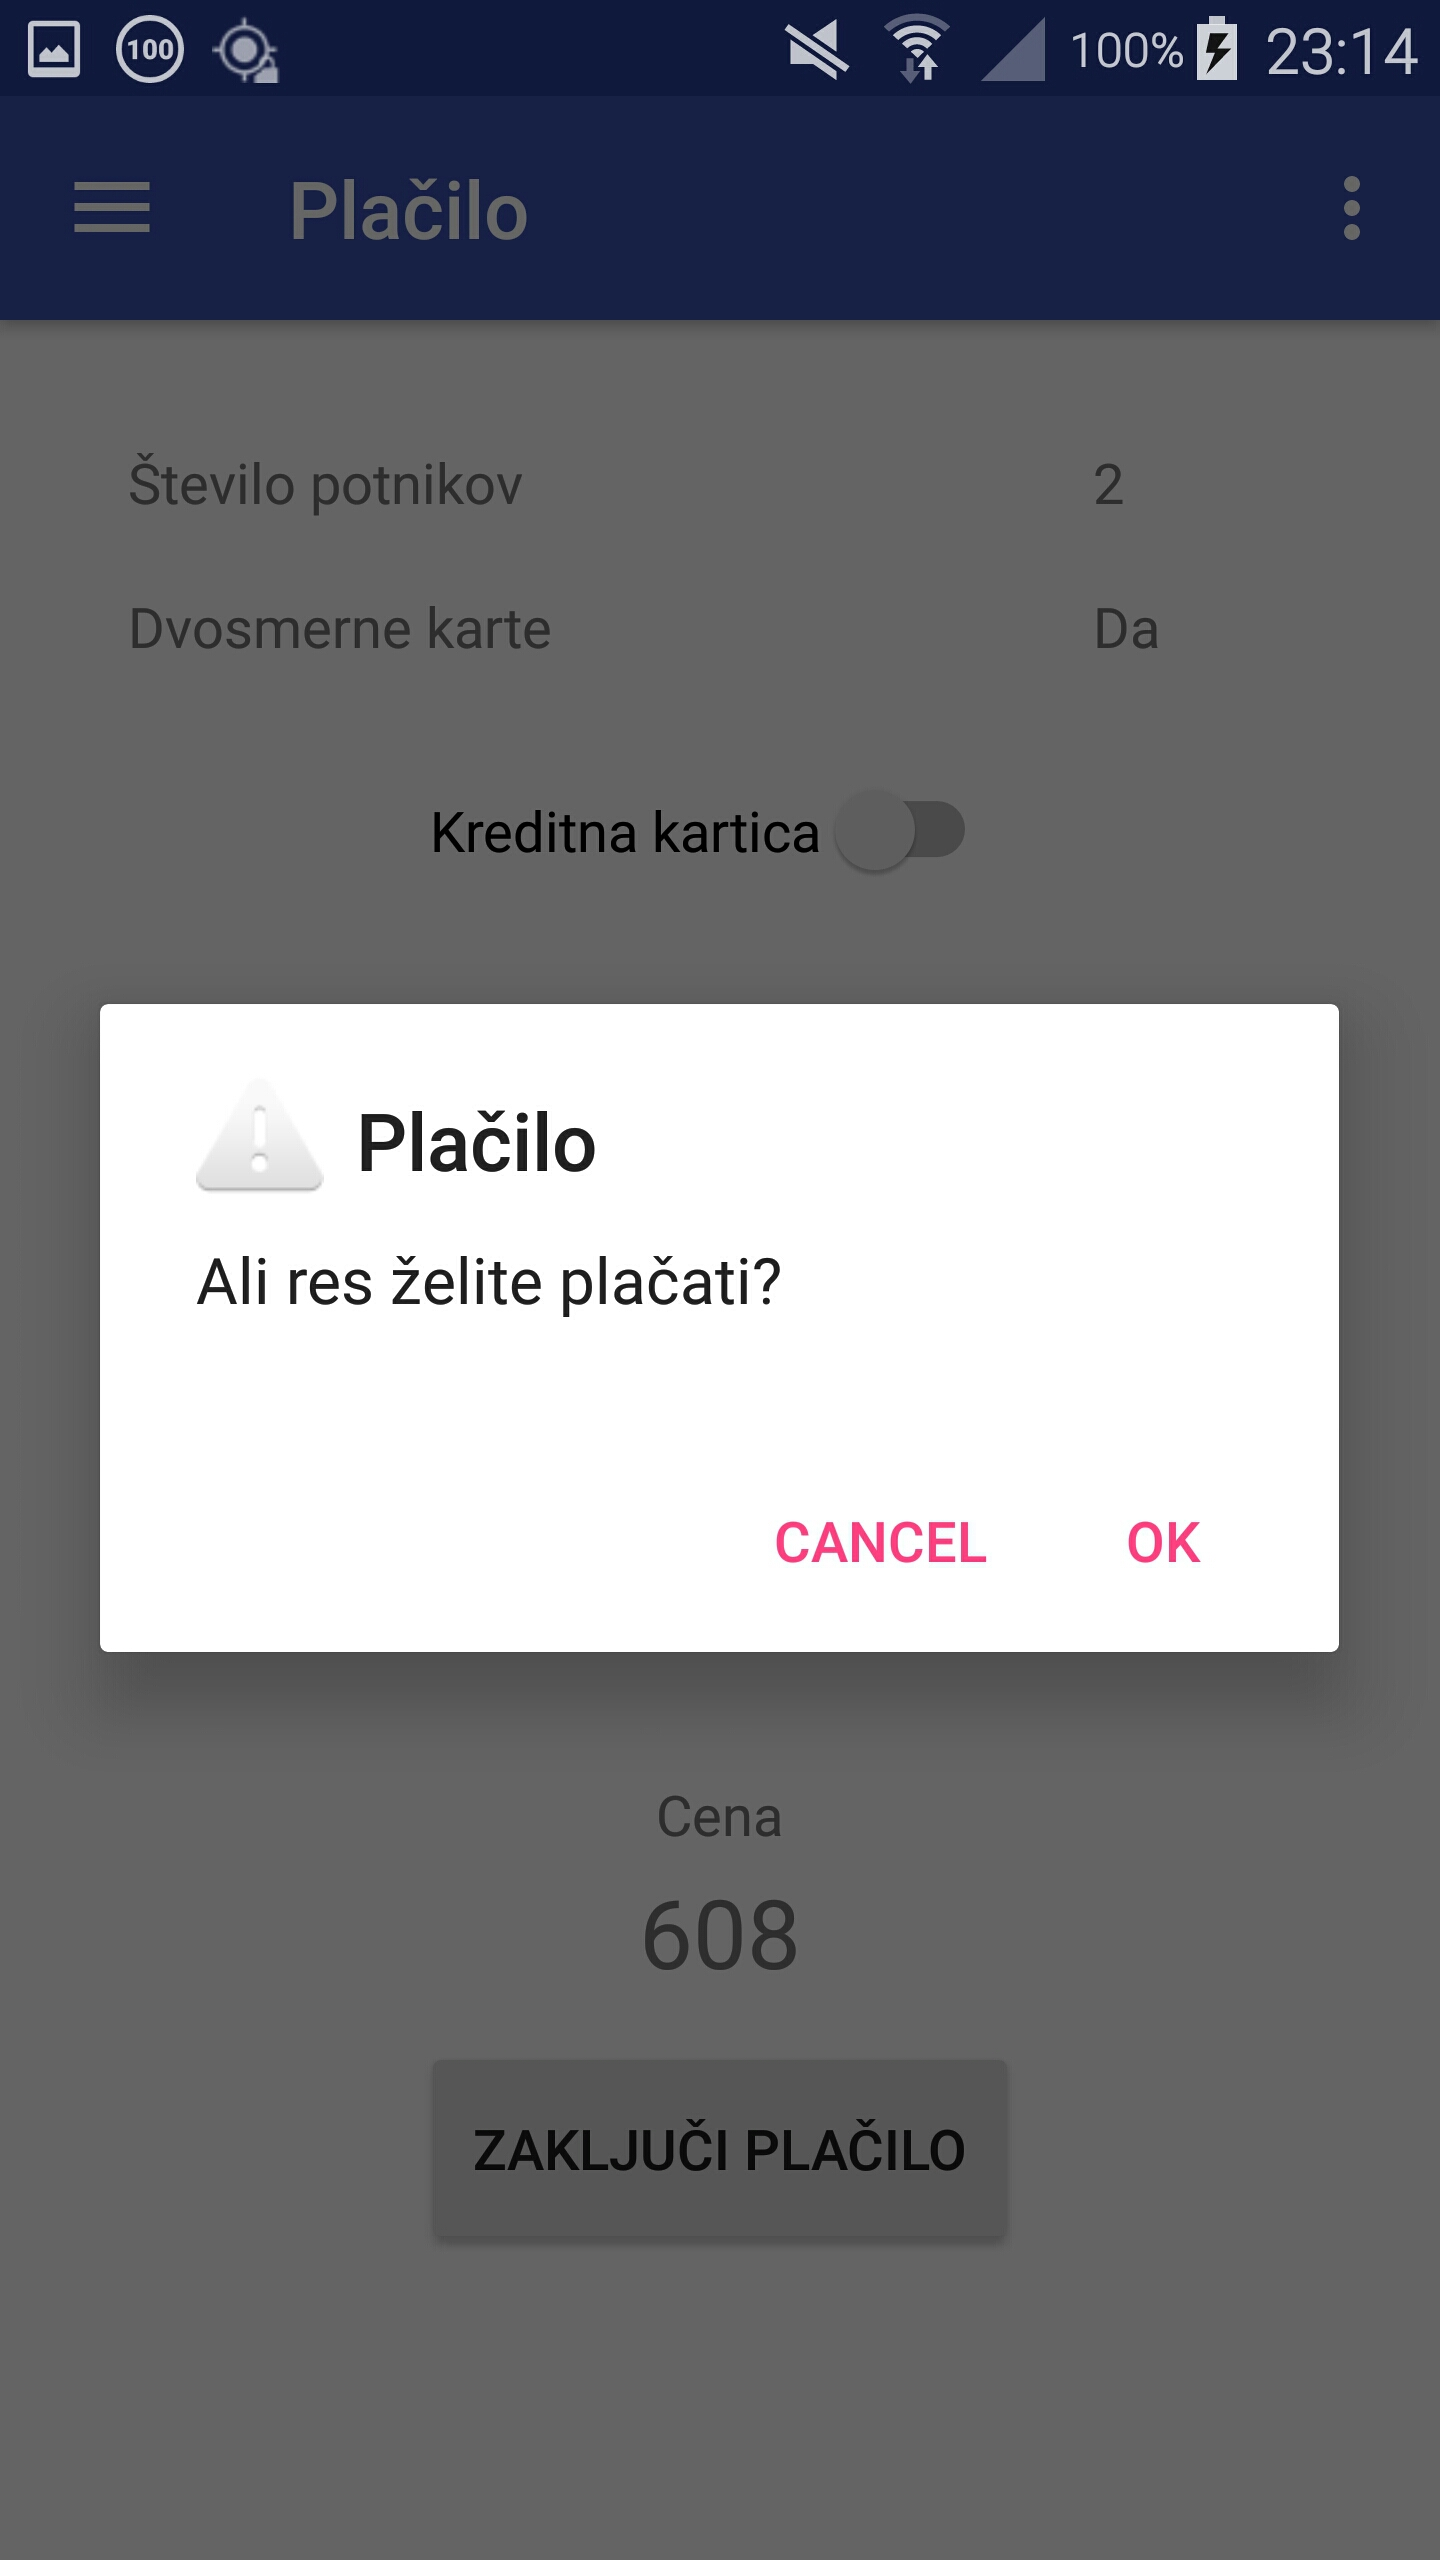
\includegraphics[width=1.0\textwidth]{GUI/zakljucekPlacila.jpg}}
	\caption{Zaključek plačila}
	\label{sl:koncept}
\end{figure}

\begin{figure}[htb]
	\centerline{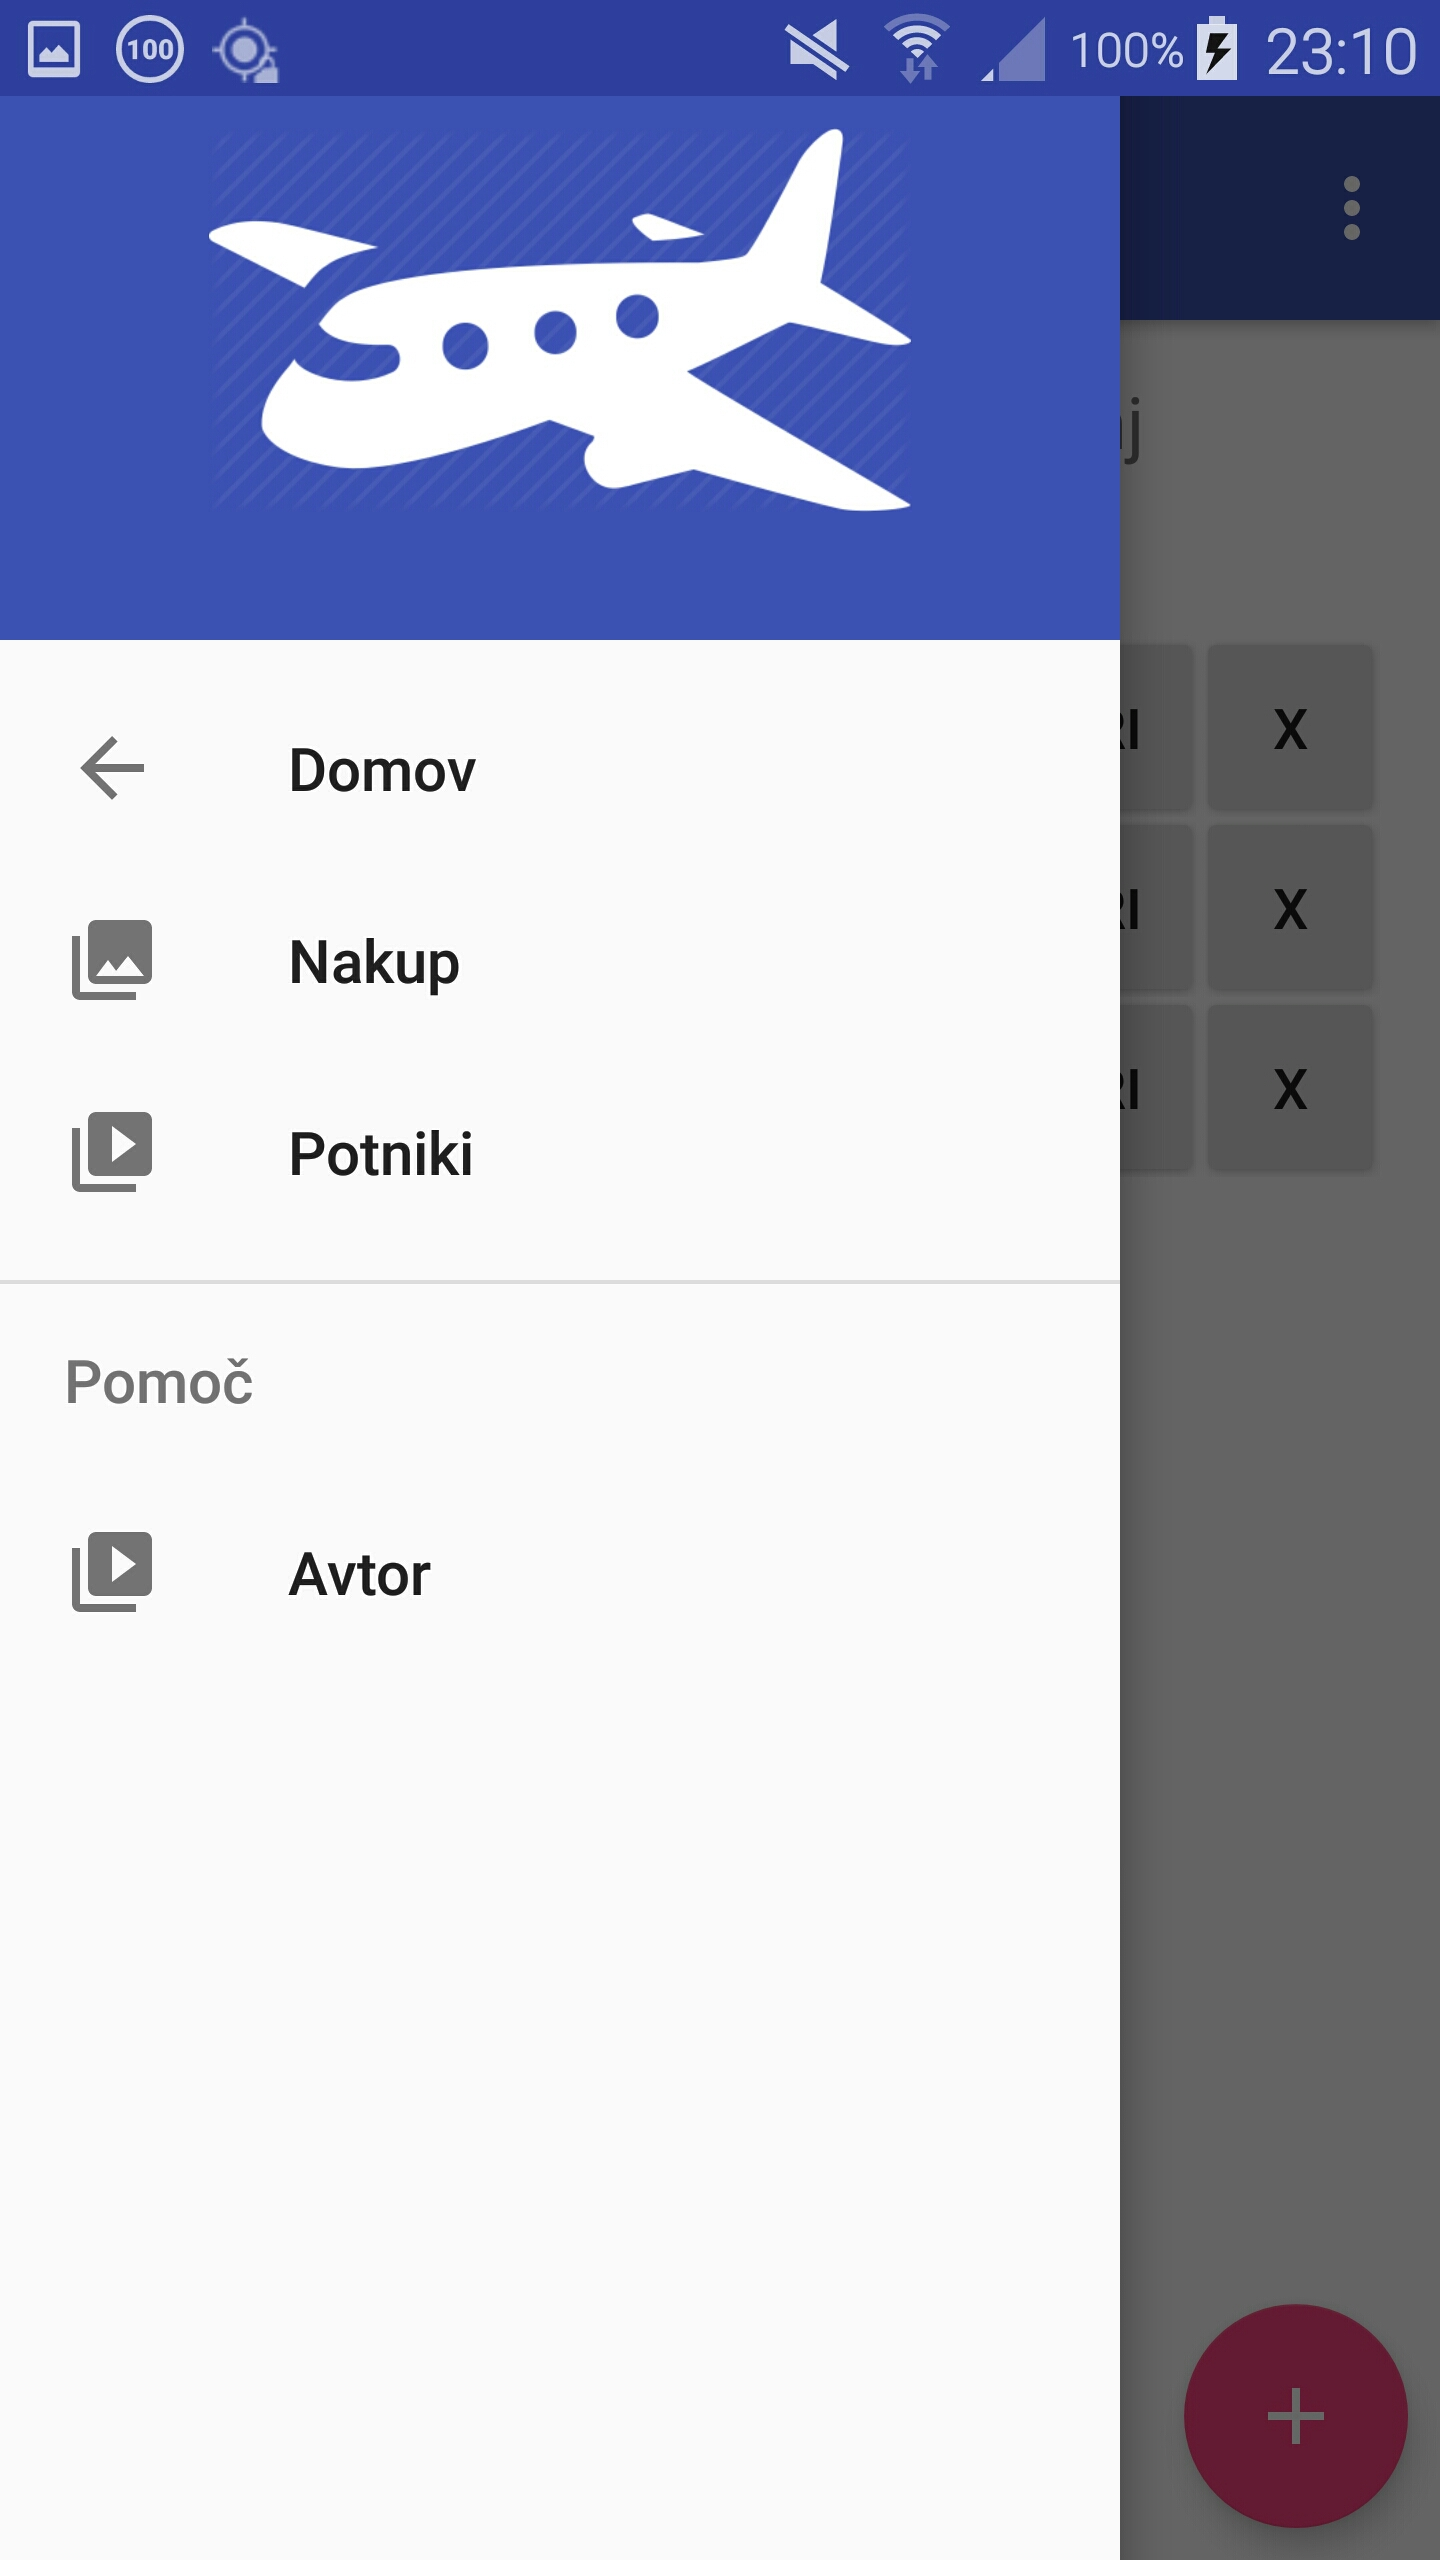
\includegraphics[width=1.0\textwidth]{GUI/navigation.jpg}}
	\caption{Navigacijsko okno}
	\label{sl:koncept}
\end{figure}

\begin{figure}[htb]
	\centerline{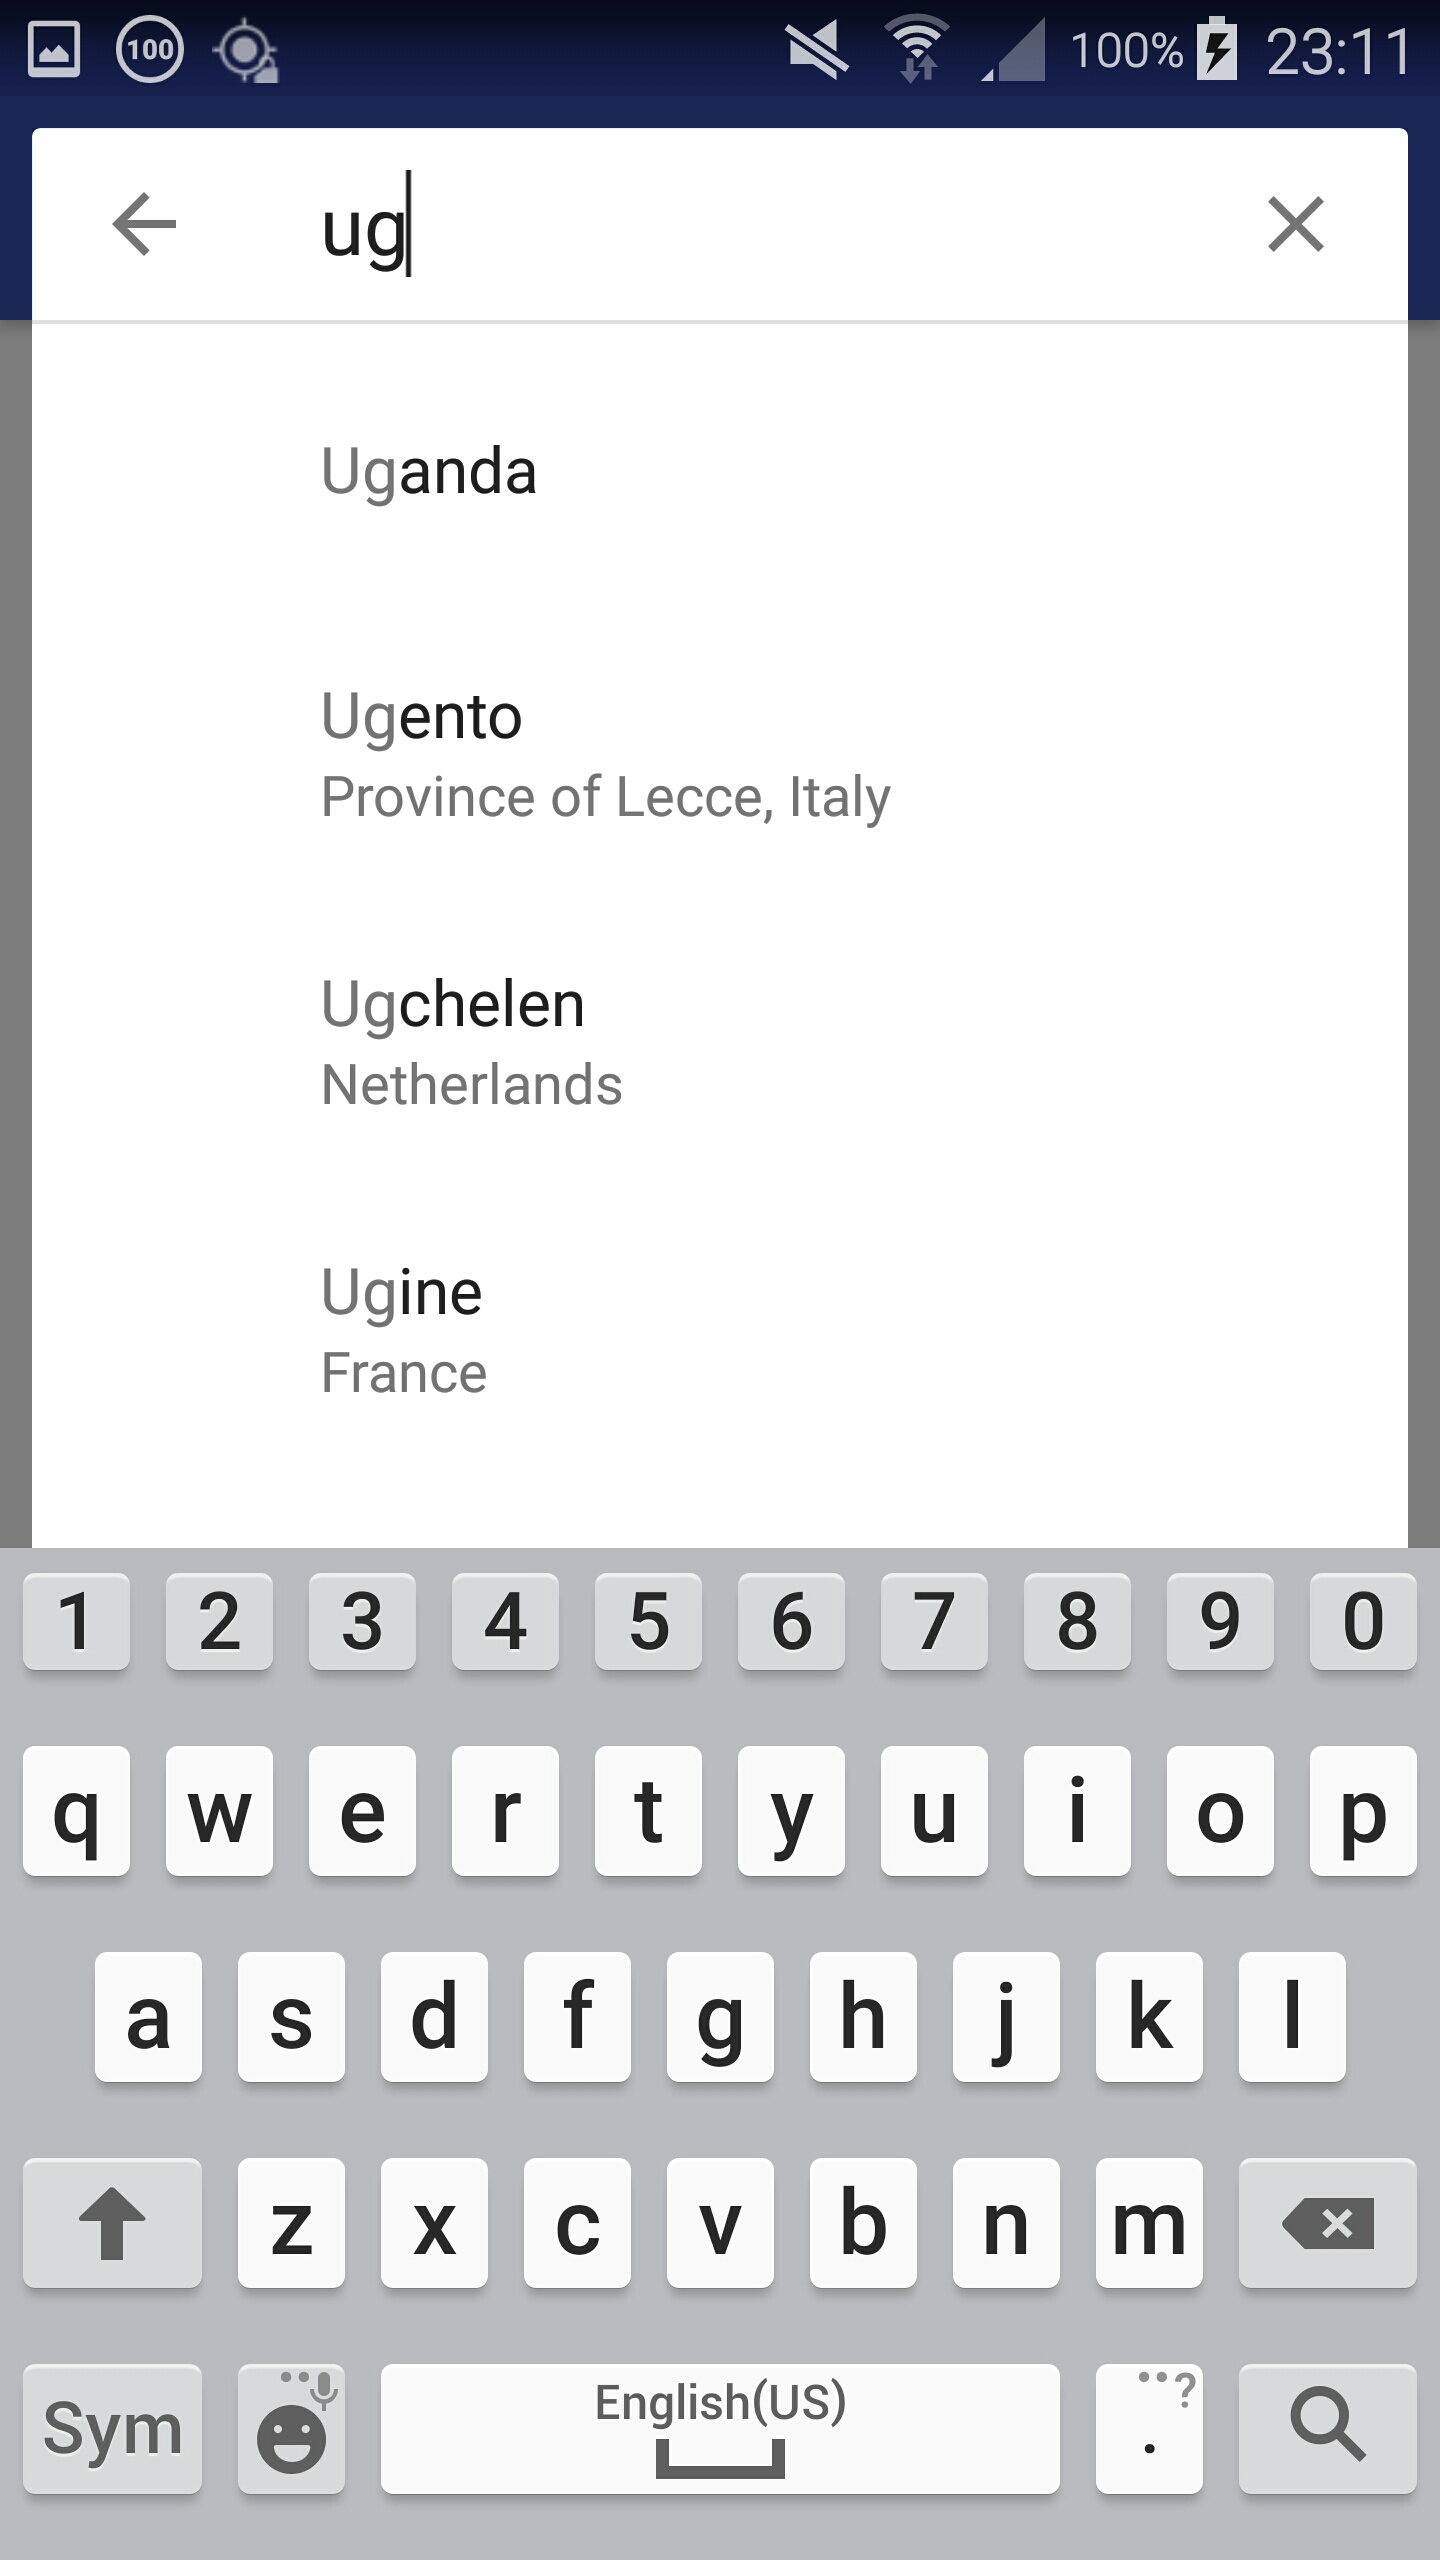
\includegraphics[width=1.0\textwidth]{GUI/autocomplete.jpg}}
	\caption{Google autocomplete fragment}
	\label{sl:koncept}
\end{figure}

\begin{figure}[htb]
	\centerline{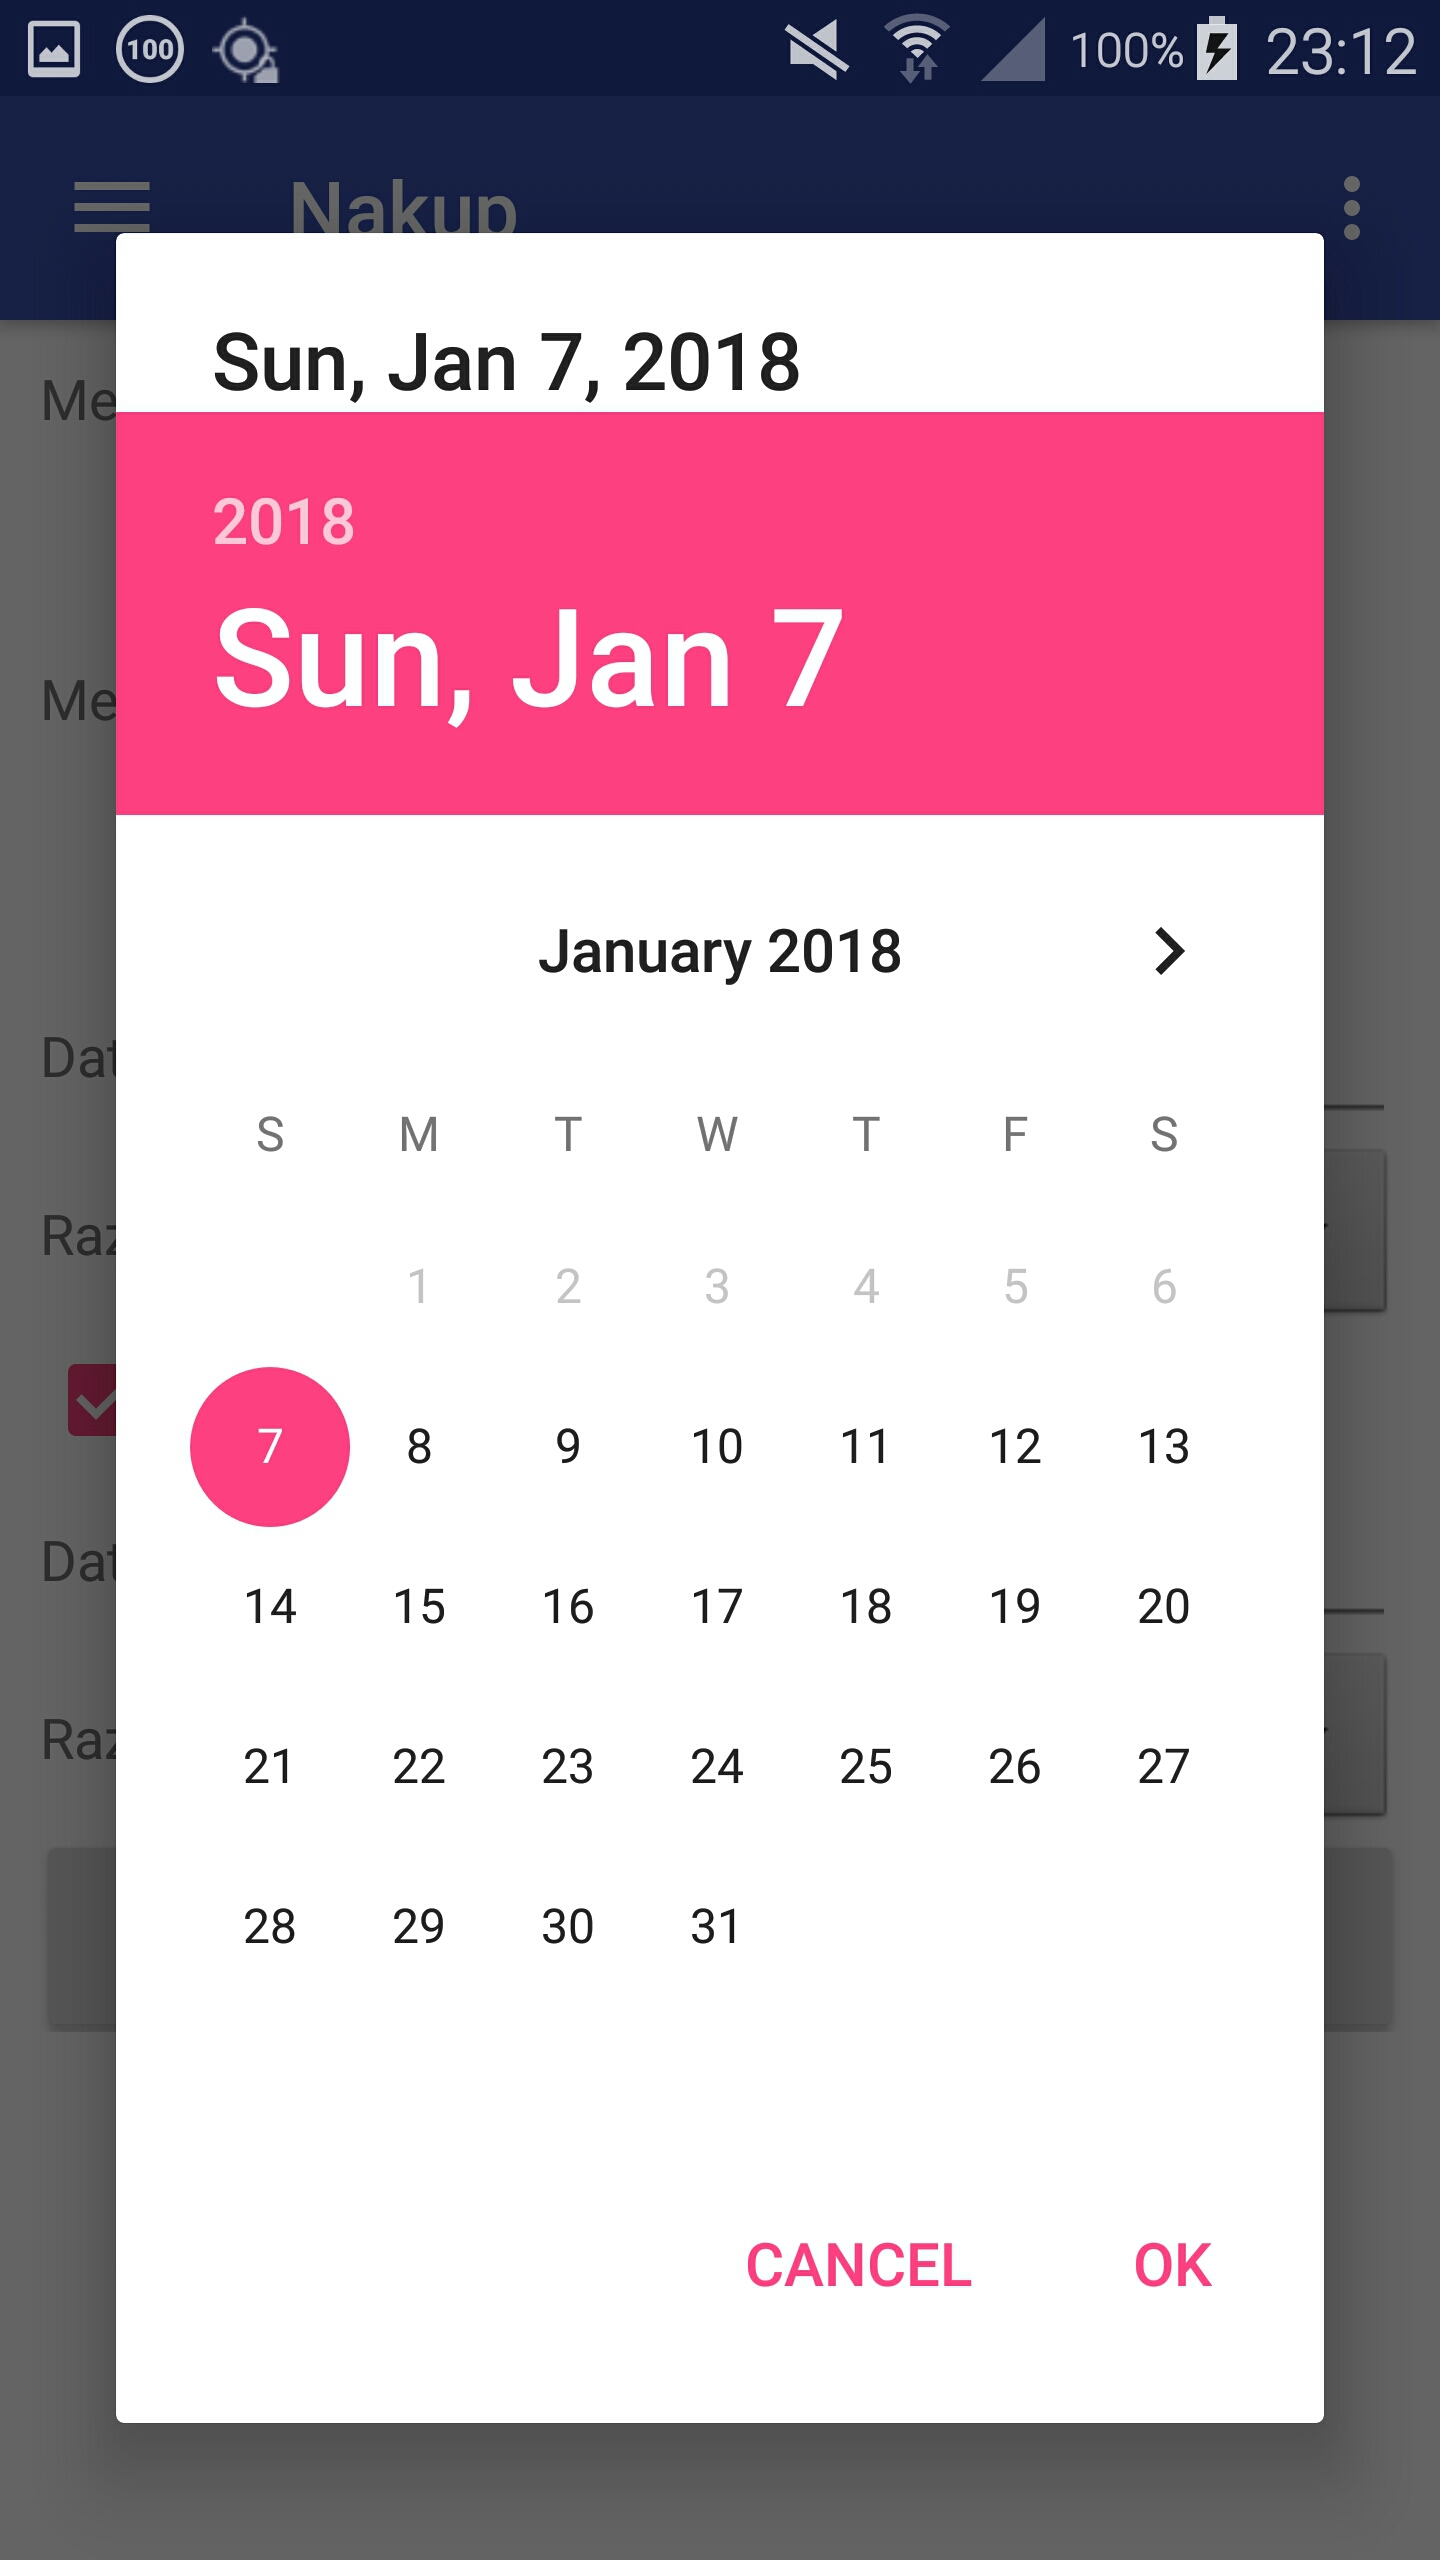
\includegraphics[width=1.0\textwidth]{GUI/datePicker.jpg}}
	\caption{Date Picker}
	\label{sl:koncept}
\end{figure}





\bibliographystyle{plain}
\bibliography{literatura}

\end{document}  




